\section{Estado da Arte do \acrshort{clav}}

Quando esta dissertação teve início o projeto \acrshort{clav} já tinha cerca de 2 anos de desenvolvimento. Assim nesta secção será apresentado o estado da arte do \acrshort{clav} quando esta dissertação iniciou aprofundando principalmente os pontos mais importantes sobre o tema desta dissertação.

\subsection{Estrutura}
A \acrshort{clav} está dividido em duas partes:
\begin{itemize}
    \item interface (\textit{front-end}) presente em \url{http://clav.dglab.gov.pt}
    \item \acrshort{api} de dados (\textit{back-end} que inclui também duas bases de dados, \textit{GraphDB} e \textit{MongoDB}) presente em \url{http://clav-api.dglab.gov.pt}.
\end{itemize}

Cada parte encontra-se numa máquina diferente.

Através da figura~\ref{fig:clav_struct} é possível ver o possível fluxo tanto de um utilizador a aceder à interface como a de um utilizador a aceder diretamente à \acrshort{api} de dados. No primeiro caso, quando um utilizador acede o servidor da interface da \acrshort{clav} é descarregado para o lado do utilizador o ficheiro \acrshort{html} (\textit{index}) e os vários ficheiros \textit{JavaScript}, \acrshort{css} e \textit{assets} (como imagens, \acrshort{pdf}s, etc) quando necessários. O servidor da interface é nada mais que um servidor \textit{web} com recurso ao \textit{Nginx} que hospeda estes ficheiros, os quais representam a interface construída com o \textit{Vue} e o \textit{Vuetify}. Como tal o código apresenta-se todo do lado do utilizador e os pedidos à \acrshort{api} serão feitos do computador do utilizador para o servidor da \acrshort{api} de dados e não do servidor da interface para o servidor da \acrshort{api} de dados. Ou seja, o fluxo de cada um desses pedidos será igual ao fluxo no caso em que se acede diretamente a \acrshort{api} sem uso de qualquer interface.

\begin{figure}[H]
    \begin{center}
        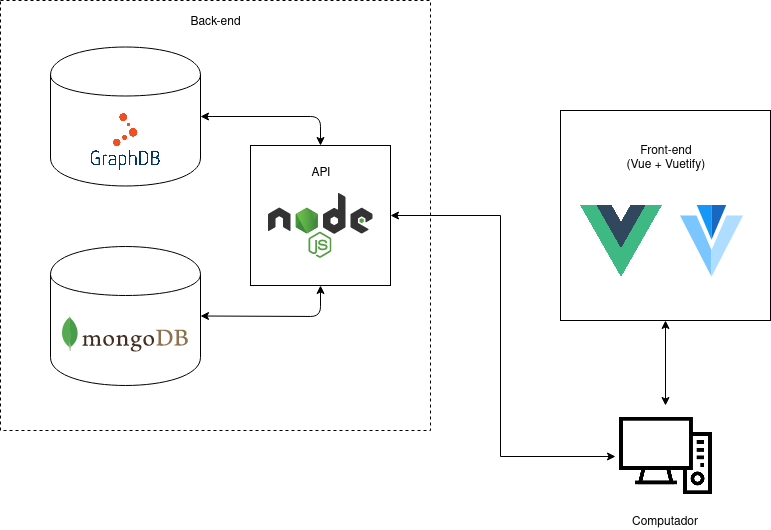
\includegraphics[width=0.7\textwidth]{img/clav_struct.png}
    \end{center}
    \caption{Estrutura da \acrshort{clav} incluindo a interação de um utilizador com a mesma}\label{fig:clav_struct}
\end{figure}

Esta estrutura evoluiu depois para a estrutura presente na figura~\ref{fig:clav_struct2} em que tanto a interface como o \textit{back-end} estão ``por trás'' do \textit{Nginx} o que leva a que todos os pedidos passem por este, seja para obter a interface (onde o \textit{Nginx} devolve esta) como para aceder a \acrshort{api} de dados (onde o \textit{Nginx} reencaminha o pedido para a \acrshort{api}).

\begin{figure}[H]
    \begin{center}
        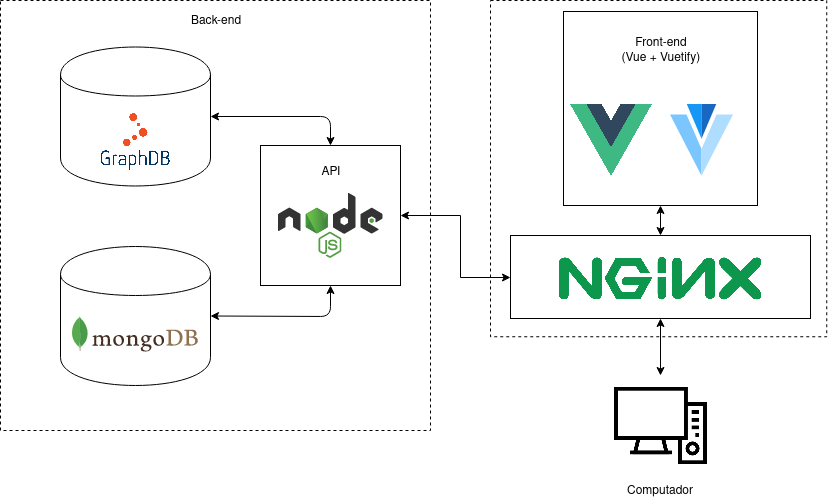
\includegraphics[width=0.7\textwidth]{img/clav_struct2.png}
    \end{center}
    \caption{Estrutura evoluída da \acrshort{clav}}\label{fig:clav_struct2}
\end{figure}

\subsection{Formas de autenticação}\label{sec:autenticacao}
A \acrshort{api} de dados e a interface estavam inicialmente ``juntas'' (aplicação monolítica) onde as rotas eram protegidas contudo, com a separação da aplicação em duas partes, ambas partes deixaram de estar protegidas. Devido à plataforma já ter estado protegida esta já possui duas formas de autenticação, através de chaves \acrshort{api} e através de utilizadores registados. Ou seja, tanto o registo de utilizadores e de chaves API já se encontra implementado bem como o \textit{login} de utilizadores.

As chaves \acrshort{api} existem por forma a dar acesso a certas rotas da \acrshort{api} a aplicações que interajam com a mesma (por exemplo sistemas de informação) sem a necessidade de interação humana.

Já os utilizadores possuem múltiplos níveis de acesso sendo que consoante o seu nível podem ou não aceder a uma rota da interface ou da \acrshort{api}. Os utilizadores podem se autenticar através de \textit{email} e \textit{password} ou com recurso ao \acrfull{cc} através do Autenticação.gov, este último apenas disponível através da interface da \acrshort{clav}.

A hierarquia dos níveis de acesso, do nível que permite menor para o maior acesso, é a seguinte:
\begin{itemize}
    \item Nível 0: Chaves API
    \item Nível 1: Representante Entidade
    \item Nível 2: Utilizador Simples
    \item Nível 3: Utilizador Avançado
    \item Nível 3.5: Utilizador Validador (\acrshort{ad})
    \item Nível 4: Utilizador Validador
    \item Nível 5: Utilizador Decisor
    \item Nível 6: Administrador de Perfil Funcional
    \item Nível 7: Administrador de Perfil Tecnológico
\end{itemize}

As chaves \acrshort{api} poderão aceder a algumas rotas com método \texttt{GET}.
Já os utilizadores poderão realizar todos os pedidos que as chaves \acrshort{api} podem realizar mas quanto maior o seu nível de acesso mais rotas poderão aceder.

A proteção da \acrshort{api} terá de ter esta hierarquia em conta.

\subsubsection{Registo}

Como já referido, tanto o registo de chaves \acrshort{api} como de utilizadores já se encontra implementado.

Para o registo de uma chave \acrshort{api} é necessário providenciar um nome, um email e a entidade a que pertence. Após o registo da chave a informação desta chave \acrshort{api} é mantida numa base de dados \textit{MongoDB}.

Um utilizador pode se registar através de \texttt{email + password} ou através do Autenticação.gov. No primeiro caso, ao se registar necessita obviamente de indicar o seu email, a \textit{password}, o seu nome, a entidade a que pertence e o nível de acesso que pretende. Já no caso do Autenticação.gov para o registo do utilizador é necessário todos os campos anteriores exceto a \textit{password} (pode ser depois definida), sendo também necessário o campo \acrfull{nic} do utilizador. Caso o registo seja efetuado com recurso à interface do Autenticação.gov apenas será necessário indicar o email, a entidade a que pertence e o nível de acesso que pretende visto que os restantes campos são fornecidos pela Autenticação.gov quando o utilizador se autentica e autoriza a partilha dessa informação com a plataforma da \acrshort{clav}.
A \textit{password} é armazenada não na sua forma literal mas sim a sua \textit{hash} ao aplicar a função criptográfica \texttt{bcrypt}. A utilização de funções de \textit{hash} criptográficas ao armazenar \textit{passwords} impede que as \textit{passwords} originais se saibam caso a base de dados seja comprometida. Para além disso, como o \texttt{bcrypt} combina um valor aleatório (\texttt{salt}) com a \textit{password} do utilizador, é impossível pré-computar a \textit{password} que deu origem ao \textit{hash} sem saber o \texttt{salt}\footnote{Para mais informação veja \textit{rainbow table attack}}.

Durante esta tese com a proteção da \acrshort{api} ficará apenas possível o registo de utilizadores através de utilizadores que já estejam registados e possuam um nível de acesso suficiente para registar utilizadores. Estes utilizadores registados e autorizados pertencem à entidade \acrshort{dglab}. Portanto por forma a utilizadores representantes de outras entidades se registarem na plataforma terão de:~\cite{clavwebpage}
\begin{itemize}
    \item Preencher o formulário disponibilizado para o efeito, para cada representante designado pela entidade;
    \item O formulário deverá ser assinado por um dirigente superior da Entidade e autenticado com assinatura digital, se o envio for feito por via eletrónica (NB\@: não serão aceites assinaturas do formulário por dirigentes intermédios). Esta autorização autenticada pelo dirigente superior é o equivalente a uma delegação de competências, uma vez que o representante da entidade passa a ter capacidade para, em nome da entidade, submeter autos de eliminação, propostas de tabelas de seleção e novas classes para a Lista Consolidada;
    \item O formulário deverá ser remetido à \acrshort{dglab} por via postal ou eletrónica, respetivamente, para:
    \begin{itemize}
        \item \acrshort{dglab}, Edifício da Torre do Tombo, Alameda da Universidade, 1649--010 Lisboa (formulário assinado manualmente) ou
        \item clav@dglab.gov.pt (formulário com assinatura digital).
    \end{itemize}
    \item Após receção do formulário, a \acrshort{dglab} efetuará o(s) respetivo(s) registo(s) até 48 horas úteis;
    \item Findo esse prazo, o utilizador poderá aceder à plataforma, selecionando a opção ``Autenticação'';
    \item A autenticação, no primeiro acesso, deve ser efetuada com o \acrlong{cc}.
\end{itemize}

\subsubsection{\textit{Login}}

O \textit{login} apenas está presente para o caso dos utilizadores visto que assim que uma chave \acrshort{api} é registada é enviado por email um \acrshort{jwt} com a duração de 30 dias a ser usado nos pedidos a realizar à \acrshort{api}. O utilizador poderá ao fim dos 30 dias renovar a sua chave \acrshort{api}, onde é gerado um novo \acrshort{jwt}.

Portanto do lado dos utilizadores é possível como já referido realizar o \textit{login} de duas formas através de uma estratégia local ou através do Autenticação.gov.

A estratégia local (\texttt{email + password}) é conseguida através do uso do \textit{middleware} \textit{Passport}.
O \textit{Passport} é um middleware de autenticação para \textit{Node.js} que tem como objetivo autenticar pedidos.~\cite{passport} Tem como única preocupação a autenticação delegando qualquer outra funcionalidade para a aplicação que a usa. Este \textit{middleware} possui muitas estratégias de autenticação entre as quais a local (\texttt{email/username + password}), \acrshort{jwt}, \textit{OAuth}\footnote{Protocolo \textit{open-source} com o objetivo de permitir a autenticação simples, segura e padrão entre aplicações móveis, \textit{web} e \textit{desktop}}, \textit{Facebook} ou \textit{Twitter}. Cada estratégia está num módulo independente. Assim as aplicações que usam o \textit{Passport} não terão um peso adicional devido a estratégias que nem sequer usam.

No caso do \textit{login} através do Autenticação.gov, o utilizador tem de se autenticar na interface do Autenticação.gov (a partir do botão disponível na área de autenticação da interface do \acrshort{clav}). O fluxo do \textit{login} neste caso é: 

\begin{figure}[H]
    \begin{center}
        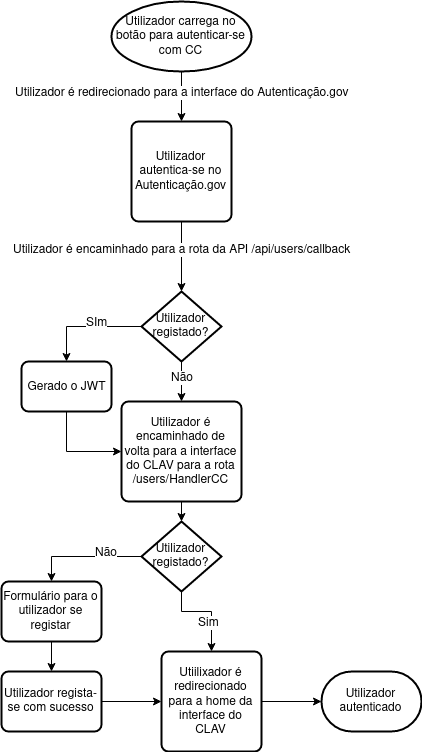
\includegraphics[width=0.5\textwidth]{img/authgov.png}
    \end{center}
    \caption{Fluxo do \textit{login} de um utilizador através do Autenticação.gov}\label{fig:authgov}
\end{figure}

No \textit{login} do utilizador é gerado um \acrshort{jwt} com a duração de 8 horas que deve ser usado nos pedidos a realizar à \acrshort{api}. No fim das 8 horas o utilizador necessita de se autenticar de novo.

%TODO
%\subsection{Lista Consolidada}

%TODO
%\subsection{Tabelas de Seleção}

%TODO
%\subsection{Cache e Fecho Transitivo}

%TODO
%\section{\acrshort{rest}}
%~\cite{restws}

%TODO
%\section{express}
%\cite{wdmongo}
%procurar "semelhantes" para cada um

\section{\acrfull{jwt}}
O \acrshort{jwt} é um \textit{open standard}\footnote{Mais informação em \url{https://tools.ietf.org/html/rfc7519}} que define uma forma compacta e independente de transmitir com segurança informação entre partes com um objeto \acrshort{json}.~\cite{jwtio} O \acrshort{jwt} pode ser assinado digitalmente (\acrshort{jws}), encriptado (\acrshort{jwe}), assinado e depois encriptado (\acrshort{jws} encriptado, ou seja, um \acrshort{jwe}, ordem recomendada\footnote{Mais informação em \url{https://tools.ietf.org/html/rfc7519\#section-11.2}}) ou encriptado e depois assinado (\acrshort{jwe} assinado, ou seja, um \acrshort{jws}).

Caso seja assinado digitalmente é possível verificar a integridade da informação mas não é garantida a sua privacidade contudo podemos confiar na informação do \acrshort{jwt}. A assinatura pode ser efetuada através de um segredo usando por exemplo o algoritmo \acrshort{hmac} ou através de pares de chaves pública/privada usando por exemplo o algoritmo \acrshort{rsa}. No caso de se usar pares de chaves pública/privada a assinatura também garante que a parte envolvida que tem a chave privada é aquela que assinou o \acrshort{jwt}.

Por outro lado, os \acrshort{jwt}s podem ser encriptados garantindo a privacidade destes, escondendo a informação das partes não envolvidas. Nesta secção apenas se falará sobre \acrshort{jwt}s e \acrshort{jws}s (\acrshort{jwt} assinado). Se pretender saber mais sobre \acrshort{jwe}s pode ler o capítulo 5 do livro \textit{The JWT Handbook} por \textit{Sebastián E. Peyrott}.

Sendo assim em que casos é útil o uso de \acrshort{jwt}s? Dois dos casos são os seguintes:
\begin{itemize}
    \item Autorização: Este será o caso para o qual o \acrshort{jwt} será usado na \acrshort{clav}. Quando o utilizador realiza o \textit{login} gera-se um \acrshort{jwt} por forma a que os restantes pedidos desse utilizador sejam realizados com esse \acrshort{jwt} (\acrlong{sso}). O uso de \acrshort{jwt}s para estes casos permitem um \textit{overhead} pequeno e a flexibilidade de serem usados em diferentes domínios.
    \item Troca de informação: No caso de troca de informação entre duas partes os \acrshort{jwt}s assinados são de bastante utilidade visto que permitem verificar se o conteúdo não foi violado e, no caso de se usar pares de chaves pública/privada para assinar, permitem ter a certeza que o remetente é quem diz ser.
\end{itemize}

\subsection{Estrutura do \acrshort{jwt}}

Os \acrshort{jwt}s são construídos a partir de três elementos, o \textit{header} (objeto \acrshort{json} também conhecido por \acrshort{jose} \textit{header}), o \textit{payload} (objeto \acrshort{json}) e os dados de assinatura/encriptação (depende do algoritmo usado). Estes elementos são depois codificados em representações compactas (\texttt{Base64 URL-safe}\footnote{Variante da codificação \texttt{Base64} onde a codificação gerada é segura para ser usada em \textit{URL}s. Basicamente para a codificação \texttt{Base64} gerada substitui os caracteres '+' e '/' pelos caracteres '-' e '\_' respetivamente. Além disso, remove o caractere de \textit{padding} e proíbe separadores de linha}). As codificações \texttt{Base64 URL-safe} de cada elemento são depois concatenadas através de pontos dando origem a uma representação final compacta do \acrshort{jwt} (\textit{JWS/JWE Compact Serialization}). Na secção~\ref{sec:criacaojwt} está presente dois diagramas referentes à construção de dois \acrshort{jwt}s sendo um deles assinado.

\begin{figure}[H]
    \centering
    \textbf{\textcolor{red}{eyJhbGciOiJIUzI1NiIsInR5cCI6IkpXVCJ9}.
        \textcolor{purple}{eyJuYW1lIjoiSm9zw6kgTWFydGlucyIsIm51bSI6ImE3ODgyMSJ9}.
        \textcolor{cyan}{tRPSYVsFI-nziRPuAjdGZLN2tUez5MtLML\_aAnPplgM}
    }
    \caption{Exemplo de representação compacta de \acrshort{jwt} (quebra de linhas por forma a melhorar leitura)}\label{fig:exemjwt}
\end{figure}

De seguida vamos aprofundar cada elemento referido:
\begin{itemize}
    \item[\textbf{\textit{Header}:}]

    O cabeçalho (a vermelho na figura~\ref{fig:exemjwt}) consiste nos seguintes atributos:
    \begin{itemize}
        \item O atributo obrigatório (único campo obrigatório para o caso de um \acrshort{jwt} não encriptado) \texttt{alg} (algoritmo) onde é indicado que algoritmo é usado para assinar e/ou desencriptar. O seu valor pode ser por exemplo HS256 (\acrshort{hmac} com o auxilio do SHA-256\footnote{Função pertencente ao conjunto de funções \textit{hash} criptográficas \acrfull{sha2} desenhadas pela \acrshort{nsa}}) ou \acrshort{rsa}.
        \item O atributo opcional \texttt{typ} (tipo do \textit{token}) em que o seu valor é ``JWT''. Serve apenas para distinguir os \acrshort{jwt}s de outros objetos que têm um \acrshort{jose} \textit{header}.
        \item O atributo opcional \texttt{cty} (tipo do conteúdo (\textit{payload})). Se o \textit{payload} conter atributos arbitrários este atributo não deve ser colocado. Caso o \textit{payload} seja um \acrshort{jwt}\footnote{\acrshort{jwt} aninhado (\textit{nested \acrshort{jwt}})} então este atributo deve ter o valor de ``JWT''.
    \end{itemize}

    O cabeçalho é de grande importância visto que permite saber se o \acrshort{jwt} é assinado ou encriptado e de que forma o resto do \acrshort{jwt} deve ser interpretado.

    \begin{lstlisting}[language=json, caption=\textit{Header} usado para construir o \acrshort{jwt} da figura~\ref{fig:exemjwt}]
    {
        "alg": "HS256",
        "typ": "JWT"
    }
    \end{lstlisting}

    \item [\textbf{\textit{Payload}:}] O \textit{payload} (a roxo na figura~\ref{fig:exemjwt}) contém a informação/dados que pretendemos transmitir com o \acrshort{jwt}. Não há atributos obrigatórios contudo existem certos atributos que têm um significado definido (atributos registados).

    Existem 7 atributos registados (\textit{registered claims}):~\cite{jwthandbook}
    \begin{itemize}
        \item \texttt{iss} (\textit{issuer}): Identificador único (\textit{case-sensitive string}) que identifica unicamente quem emitiu o \acrshort{jwt}. A sua interpretação é específica a cada aplicação visto que não há uma autoridade central que gere os emissores.
        \item \texttt{sub} (\textit{subject}): Identificador único (\textit{case-sensitive string}) que identifica unicamente de quem é a informação que o \acrshort{jwt} transporta. Este atributo deve ser único no contexto do emissor, ou se tal não for possível, globalmente único. O tratamento do atributo é específico a cada aplicação. 
        \item \texttt{aud} (\textit{audience}): Identificador único (\textit{case-sensitive string}) ou \textit{array} destes identificadores únicos que identificam unicamente os destinatários pretendidos do \acrshort{jwt}. Ou seja, quem lê o \acrshort{jwt} se não estiver no atributo \texttt{aud} não deve considerar os dados contidos no \acrshort{jwt}. O tratamento deste atributo também é específico a cada aplicação. 
        \item \texttt{exp} (\textit{expiration (time)}): Um número inteiro que representa uma data e hora específica no formato \textit{seconds since epoch} definido pela \acrshort{posix}\footnote{Mais informação em \url{https://pubs.opengroup.org/onlinepubs/9699919799/basedefs/V1\_chap04.html\#tag\_04\_16}}, a partir da qual o \acrshort{jwt} é considerado inválido (expira).
        \item \texttt{nbf} (\textit{not before (time)}): Representa o inverso do atributo \texttt{exp} visto que é um número inteiro que representa uma data e hora específica no mesmo formato do atributo \texttt{exp}, mas que a partir da qual o \acrshort{jwt} é considerado válido.
        \item \texttt{iat} (\textit{issued at (time)}): Um número inteiro que representa uma data e hora especifica no mesmo formato dos atributos \texttt{exp} e \texttt{nbf} na qual o \acrshort{jwt} foi emitido.
        \item \texttt{jti} (\textit{\acrshort{jwt} ID}): Identificador único (\textit{string}) do \acrshort{jwt} que permite distinguir \acrshort{jwt}s com conteúdo semelhante. A implementação tem de garantir a unicidade deste identificador.
    \end{itemize}

    Estes atributos registados têm todos 3 caracteres visto que um dos requisitos do \acrshort{jwt} é ser o mais pequeno/compacto possível.

    Existem depois mais dois tipos de atributos, públicos e privados. Os atributos públicos podem ser definidos à vontade pelos utilizadores de \acrshort{jwt}s mas têm de ser registados em \textit{IANA JSON Web Token Claims registry} ou definidos por um espaço de nomes resistente a colisões de forma a evitar a colisão de atributos. Já os atributos privados são aqueles que não são nem registados nem públicos e podem ser definidos à vontade pelos utilizadores de \acrshort{jwt}s. Os dois atributos usados no exemplo~\ref{exem:pay} (\texttt{name} e \texttt{num}) são atributos privados.

    \begin{lstlisting}[language=json, caption=\textit{Payload} usado para construir o \acrshort{jwt} da figura~\ref{fig:exemjwt}, label=exem:pay]
    {
        "name": "José Martins",
        "num": "a78821"
    }
    \end{lstlisting}

\item [\textbf{\textit{Signature}:}] A assinatura (a azul na figura~\ref{fig:exemjwt}) é criada ao usar o algoritmo indicado na \textit{header} no atributo \texttt{alg} tendo como um dos argumentos os elementos codificados da \textit{header} e do \textit{payload} juntos por um ponto e como outro argumento um segredo. O resultado do algoritmo é depois codificado em \texttt{Base64 URL-safe}. Esta assinatura no caso dos \acrshort{jws}s é usada para verificar a integridade do \acrshort{jwt} e caso seja assinado com uma chave privada permite também verificar se o remetente é quem diz ser. No caso de o atributo \texttt{alg} for \texttt{none} a assinatura é uma \texttt{string} vazia.

    \begin{lstlisting}[language=javascript, caption=\textit{Signature} usado para construir o \acrshort{jwt} da figura~\ref{fig:exemjwt}]
    HMACSHA256(
        base64UrlEncode(header) + "." +
        base64UrlEncode(payload),
        segredo1.-uminho!clav
    )
    \end{lstlisting}
\end{itemize}

\subsection{Criação de \acrshort{jwt}/\acrshort{jws}}\label{sec:criacaojwt}

Na figura~\ref{fig:buildJWT} é apresentada a construção de um \acrshort{jwt} em que o atributo \texttt{alg} (algoritmo) tem o seu valor igual a \texttt{none}, ou seja, o \acrshort{jwt} não é assinado nem encriptado.

\begin{figure}[H]
    \begin{center}
        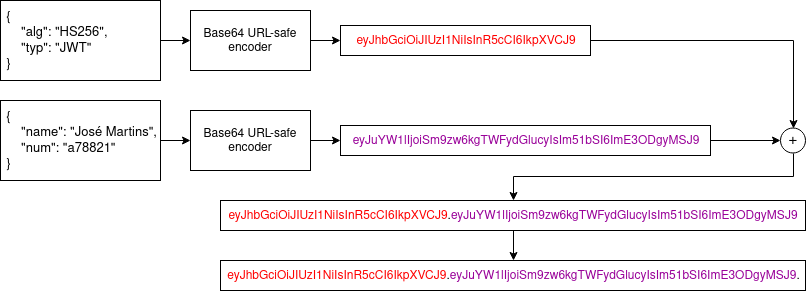
\includegraphics[width=1\textwidth]{img/buildJWT.png}
    \end{center}
    \caption{Criação de um \acrshort{jwt}}\label{fig:buildJWT}
\end{figure}

Já na figura~\ref{fig:buildJWS} é demonstrada a construção de um \acrshort{jwt} assinado, ou seja, um \acrshort{jws}.

\begin{figure}[H]
    \begin{center}
        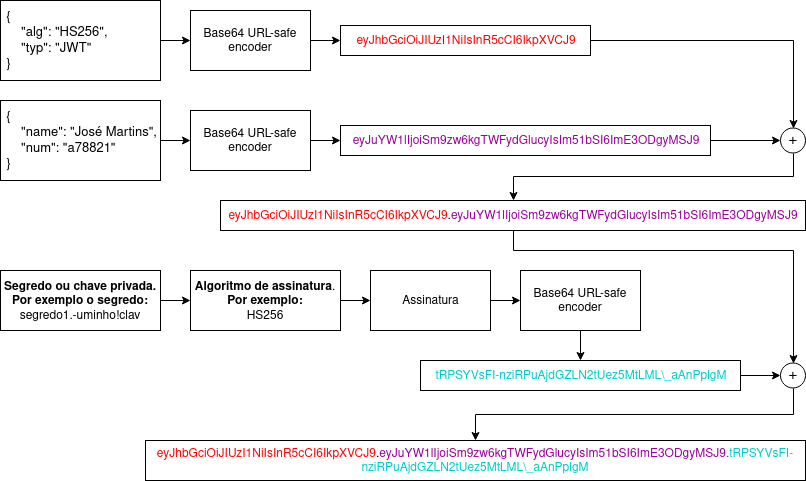
\includegraphics[width=1\textwidth]{img/buildJWS.png}
    \end{center}
    \caption{Criação de um \acrshort{jws}}\label{fig:buildJWS}
\end{figure}

\subsection{Alternativas ao \acrshort{jwt}}

Algumas alternativas ao \acrshort{jwt} passam pelo uso de \acrfull{swt} ou \acrfull{saml}. Se compararmos o \acrshort{jwt} ao \acrshort{saml}, o \acrshort{json} é menos verboso que o \acrshort{xml} e mesmo quando codificado o seu tamanho é menor. 

De um ponto de vista de segurança o \acrshort{swt} apenas pode ser assinado simetricamente por um segredo partilhado usando o algoritmo \acrshort{hmac}. Já o \acrshort{jwt} e o \acrshort{saml} podem usar pares de chaves pública/privada para assinar. Contudo assinar \acrshort{xml} com \textit{\acrshort{xml} Digital Signature} sem introduzir buracos de segurança é mais difícil quando comparado com a simplicidade de assinar \acrshort{json}.~\cite{jwtio}

Houve contudo algumas bibliotecas de \acrshort{jwt} com vulnerabilidades devido ao atributo \texttt{alg} da \textit{header} do \acrshort{jwt}. Havia duas situações de vulnerabilidade:
\begin{itemize}
    \item As bibliotecas ao fazer a verificação (recebe um \acrshort{jwt} e um segredo/chave pública como argumentos) de um \acrshort{jwt} com \texttt{alg} igual a \texttt{none} assumiam logo que o \acrshort{jwt} era válido mesmo que o segredo/chave pública fosse diferente de vazio. Ou seja, com a simples alteração do atributo \texttt{alg} e com a remoção da \textit{signature} podia-se alterar o \textit{payload} do \acrshort{jwt} que o servidor iria continuar a considerar que a integridade do \acrshort{jwt} não foi colocada em causa mesmo que os \acrshort{jwt}s gerados pelo servidor tivessem sido com um algoritmo e com recurso a um segredo/chave privada.
    \item As bibliotecas ao fazer a verificação seja um algoritmo simétrico ou assimétrico apenas tinham como parâmetros o \acrshort{jwt} e o segredo/chave pública. Isto gera uma segunda vulnerabilidade, se o servidor estiver à espera de um \acrshort{jwt} assinado com pares de chaves pública/privada mas recebe um \acrshort{jwt} assinado com \acrshort{hmac} vai assumir que a chave pública é o segredo a usar no algoritmo \acrshort{hmac}. Ou seja, se se criar um \acrshort{jwt} com o atributo \texttt{alg} igual a \acrshort{hmac} e a assinatura for gerada usando o algoritmo \acrshort{hmac} com o segredo a ser a chave pública, podemos alterar o \textit{payload} (antes de assinar) que o servidor vai considerar que o \acrshort{jwt} não foi maliciosamente alterado.
\end{itemize}

Portanto a flexibilidade de algoritmos dada pelo \acrshort{jwt} coloca em causa a segurança pelo que da parte das bibliotecas o atributo \texttt{alg} não deve ser considerado~\cite{jwtvuln} bem como deve ser \textit{deprecated} e deixar de ser incluído nos \acrshort{jwt}s\footnote{Ver \url{https://gist.github.com/paragonie-scott/c88290347c2589b0cd38d8bb6ac27c03}}. 

A biblioteca que será usada na \acrshort{clav}, \texttt{jsonwebtoken}\footnote{Ver \url{https://www.npmjs.com/package/jsonwebtoken}}, já endereçou estes problemas\footnote{Ver \url{https://github.com/auth0/node-jsonwebtoken/commit/1bb584bc382295eeb7ee8c4452a673a77a68b687}} pelo que estas vulnerabilidades não estarão presentes na \acrshort{clav}.

Ainda comparando as diferentes alternativas, os \textit{parsers} de \acrshort{json} são mais comuns em grande parte das linguagens de programação visto que os \acrshort{json}s mapeiam diretamente para objetos ao contrário do \acrshort{xml} que não tem um mapeamento natural de documento para objeto.~\cite{jwtio} Portanto isto torna mais fácil trabalhar com \acrshort{jwt} do que com \acrshort{saml}.

Já quando comparamos os \acrshort{jwt}s a \textit{cookie sessions}, o \acrshort{jwt} tem a vantagem de as sessões puderem ser \textit{stateless} enquanto que as \textit{cookies} são \textit{statefull}. Contudo, ser \textit{stateless} não permite por exemplo que a qualquer altura se possa revogar um \acrshort{jwt}. Para endereçar esse problema é necessário, por exemplo, guardar (\textit{statefull}) os \acrshort{jwt}s numa base de dados associando cada \acrshort{jwt} ao identificador único de quem é a informação contida no \acrshort{jwt} (o uso de uma \textit{whitelist}). Assim para revogar um \acrshort{jwt} bastaria removê-lo da base de dados.

Outra alternativa ao \acrshort{jwt} seria \textit{sessionIDs}. As \textit{sessionIDs} são \textit{strings} longas, únicas e aleatórias. É possível revogar um \textit{sessionID}, ao contrário do \acrshort{jwt}, bastando para isso remover o \textit{sessionID} da base de dados.

Por fim, uma outra alternativa bastante semelhante ao \acrshort{jwt} é \textit{Branca}. \textit{Branca} usa o algoritmo simétrico \textit{\acrshort{ietf} XChaCha20-Poly1305 \acrshort{aead}} que permite criar \textit{tokens} encriptados e que garantem integridade. Tem também uma região de \textit{payload} como \acrshort{jwt} com a única diferença é que este \textit{payload} não tem um estrutura definida. Não necessita da \textit{header} visto que o algoritmo usado não varia. Em vez de usar codificação em \texttt{Base64 URL-safe} usa \texttt{Base62} que também é \textit{URL-safe}. Para além disso o \textit{token} gerado é geralmente de menor dimensão do que o gerado pelo \acrshort{jwt} sendo como tal mais compacto que o \acrshort{jwt}.~\cite{branca} Visto que o \textit{Branca} encripta e garante integridade de uma forma mais simples que o \acrshort{jwt} permite (para isso era necessário recorrer a um \acrshort{jwe} que tem no seu \textit{payload} um \acrshort{jws}), sendo como tal propenso a menos erros de programação. Contudo, o \textit{Branca} ainda não é muito conhecido nem um \textit{standard} da indústria, ao contrário do \acrshort{jwt}, mas não deixa de ser algo a ter em conta para o futuro. 

\section{Autorização de pedidos à \acrshort{api}}

Quanto à forma como os pedidos serão feitos à \acrshort{api} poderão ser feitos de duas formas, através da \textit{header} \acrshort{http} \textit{Authorization} ou através da \textit{query string} do pedido em um dos seguintes campos:
\begin{itemize}[leftmargin=3cm]
    \item[\textbf{\texttt{token}}] caso seja o \texttt{token} de um utilizador:\newline
        \verb|http://example.com/path/page?token=<token>|
    \item[\textbf{\texttt{apikey}}] caso seja uma Chave \acrshort{api}:\newline
        \verb|http://example.com/path/page?apikey=<Chave API>|
\end{itemize}

Na \textit{header} \textit{Authorization} irá ser usado o esquema de autenticação \textit{Bearer}\footnote{Mais informação em \url{https://tools.ietf.org/html/rfc6750}} com umas pequenas alterações. Portanto o conteúdo da \textit{header} \textit{Authorization}:
\begin{itemize}[leftmargin=2cm]
    \item Caso seja o \texttt{token} de um utilizador é:\newline
        \verb|token <token>|
    \item Caso seja uma Chave \acrshort{api} é:\newline
        \verb|apikey <Chave API>|
\end{itemize}
ao invés do esquema de autenticação predefinido do \textit{Bearer}: \verb|Bearer <token/Chave API>|

Convém referir que a Chave \acrshort{api} é também um \textit{token}. A divisão entre utilizadores e chaves \acrshort{api} permite uma mais fácil gestão dos \textit{tokens} recebidos pela \acrshort{api} bem como usar duas formas diferentes de os gerar/verificar com o possível benefício de melhorar a segurança da \acrshort{api}.

Os \textit{token}s gerados pela \acrshort{api} serão \acrshort{jwt}s. Contudo poderiam ser outro tipo de \textit{tokens} (por exemplo uma \textit{string} aleatória e única) que o processo de envio dos \textit{tokens} para a \acrshort{api} manter-se-ia igual. 

Após descrito como poderão ser feitos os pedidos à \acrshort{api}, irá ser apresentado possíveis fluxos de interação entre utilizadores (\textit{browser}, \textit{app}, etc) e o servidor da \acrshort{api}. 

O fluxo de autenticação de um utilizador na \acrshort{api} a ser implementado será o seguinte:
\begin{figure}[H]
    \begin{center}
        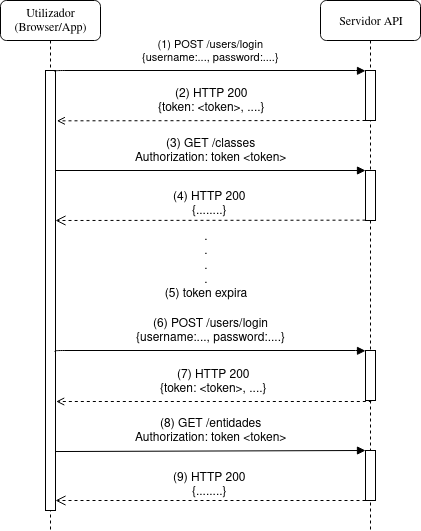
\includegraphics[width=0.5\textwidth]{img/userAuth.png}
    \end{center}
    \caption{Fluxo de autenticação e posteriores pedidos de um utilizador}\label{fig:userAuth}
\end{figure}

\begin{enumerate}
    \item Utilizador autentica-se ao providenciar o seu \textit{email} e a sua \textit{password}
    \item Caso o utilizador se autentique com sucesso é devolvido um \textit{token} que deve ser usado nos restantes pedidos até expirar
    \item Utilizador realiza um pedido para obter as classes, colocando o token na \textit{header} \textit{Authorization}
    \item Caso o \textit{token} enviado seja válido e não tenha expirado são devolvidas as classes
    \item \textit{Token} expirou após o tempo definido
    \item Utilizador realiza uma nova autenticação por forma a obter um novo \textit{token}
    \item Caso o utilizador se autentique com sucesso é devolvido um \textit{token} que deve ser usado nos restantes pedidos até expirar
    \item Utilizador realiza um pedido para obter as entidades, colocando o token na \textit{header} \textit{Authorization}
    \item Caso o \textit{token} enviado seja válido e não tenha expirado são devolvidas as entidades
\end{enumerate}

O fluxo de autenticação e renovação de uma Chave \acrshort{api} na \acrshort{api} a ser implementado será o seguinte:
\begin{figure}[H]
    \begin{center}
        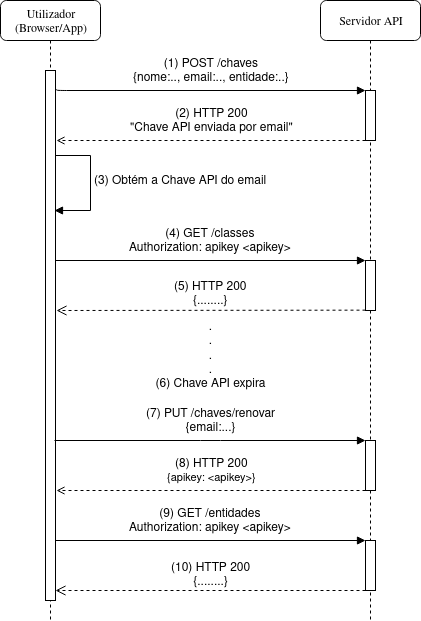
\includegraphics[width=0.5\textwidth]{img/chaveAuth.png}
    \end{center}
    \caption{Fluxo de autenticação e posteriores pedidos de uma chave \acrshort{api}}\label{fig:chaveAuth}
\end{figure}

\begin{enumerate}
    \item Utilizador cria uma chave \acrshort{api} ao providenciar o nome, email e entidade
    \item A Chave \acrshort{api} é enviada para o email fornecido pelo utilizador com o objetivo de ser usada nos próximos pedidos
    \item O utilizador obtém a chave \acrshort{api} do email enviado
    \item Utilizador realiza um pedido para obter as classes, colocando a chave \acrshort{api} na \textit{header} \textit{Authorization}
    \item Caso a Chave \acrshort{api} enviada seja válida e não tenha expirado são devolvidas as classes
    \item Chave \acrshort{api} expirou após o tempo definido
    \item Utilizador renova a Chave \acrshort{api} ao providenciar o email usado para criar a Chave \acrshort{api}
    \item A nova (renovada) Chave \acrshort{api} é devolvida para ser usada nos restantes pedidos
    \item Utilizador realiza um pedido para obter as entidades, colocando a Chave \acrshort{api} na \textit{header} \textit{Authorization}
    \item Caso a Chave \acrshort{api} enviada seja válida e não tenha expirado são devolvidas as entidades
\end{enumerate}

\subsection{Verificação dos \textit{tokens} no servidor \acrshort{api}}

Para proteger as rotas da \acrshort{api} é necessário haver métodos de verificação dos \textit{tokens} com o objetivo de decidir se o utilizador/Chave \acrshort{api} pode aceder a uma determinada rota. De seguida será apresentado o pseudo-código de verificação dos \textit{tokens} tendo em conta que os utilizadores registados conseguem aceder a todas as rotas que as Chaves \acrshort{api} conseguem mas que o inverso não acontece. Ou seja, um utilizador registado até o de nível mais baixo por exemplo, consegue aceder a todas as rotas que as Chaves \acrshort{api} tem acesso e mais algumas nas quais as Chaves \acrshort{api} não têm permissões de acesso.

Por forma a validar se uma Chave \acrshort{api} pode aceder a uma determinada rota pode ser executada a seguinte função em \textit{middleware}:
\begin{lstlisting}[language=pseudocode, caption=Verificação se um pedido com uma determinada Chave \acrshort{api} pode ser efetuado]
function isLoggedInKey(req, res, next)
    key = getJWTfromHeaderOrQueryString('apikey')

    if key then
        keyBD = getKeyFromMongoDB(key)
        if keyBD then
            res = jwt.verify(key, secretForAPIkey)
            if res != expired then
                if keyBD.active == True then
                    return next()
                else
                    return err
            else
                return err
        else
            return err
    else
        return isLoggedInUser(req, res, next)
\end{lstlisting}
É importante destacar a chamada da função \texttt{isLoggedInUser} que é executada no caso de não ser detetado uma Chave \acrshort{api} no pedido (na \textit{header} \textit{Authorization} ou na \textit{query string} \texttt{apikey}) e como tal, com essa chamada, tenta-se perceber se afinal foi passado um \textit{token} de um utilizador já que todos os utilizadores conseguem aceder às rotas que as Chaves \acrshort{api} conseguem como já referido.

No seguimento, para validar se um determinado \textit{token} de um utilizador registado pode aceder a uma determinada rota é executada a seguinte função em \textit{middleware}:
\begin{lstlisting}[language=pseudocode, caption=Verificação se um pedido com um determinado \textit{token} de um utilizador registado pode ser efetuado]
JWTstrategy = passport-jwt.Strategy

passport.use("jwt", new JWTstrategy(
    secretOrKey: secret,
    algorithms: ["HS256"],
    jwtFromRequest: getJWTfromHeaderOrQueryString('token')
, (token, done) => done(null, token)))

function isLoggedInUser(req, res, next)
    passport.authenticate("jwt", { session: false }, function (err, user, info)
        if err then
            return err
        if !user then
            return err
        req.logIn(user, function(err)
            if err then
                return err
            
            next()
        )
    )(req, res, next)
\end{lstlisting}

Os \textit{tokens} tanto das Chaves \acrshort{api} como de \textit{tokens} de utilizadores registados são obtidos através da utilização de extratores presentes na estratégia \texttt{passport-jwt} do \texttt{passport}. Assim para extrair o \textit{token} da \textit{query string} basta:
\begin{lstlisting}[language=javascript, caption=Extração do \textit{token} da \textit{query string}]
var ExtractJWT = require("passport-jwt").ExtractJwt
token = ExtractJWT.fromUrlQueryParameter("<nome do campo, 'token' ou 'apikey' no caso da CLAV>")
\end{lstlisting}
Já para extrair o \textit{token} da \textit{header} \textit{Authorization} basta:
\begin{lstlisting}[language=javascript, caption=Extração do \textit{token} da \textit{heaer} \textit{Authorization}]
var ExtractJWT = require("passport-jwt").ExtractJwt
token = ExtractJWT.fromAuthHeaderWithScheme("<palavra antes do token, 'Bearer' no caso dum bearer token, 'token' ou 'apikey' no caso da CLAV>")
\end{lstlisting}

Para verificar se o utilizador registado tem um nível suficiente para aceder a uma rota, depois de se verificar que o utilizador está autenticado (\texttt{isLoggedInUser}), deve-se executar também em \textit{middleware} a seguinte função:
\begin{lstlisting}[language=pseudocode, caption=Verificação se um utilizador registado tem permissões suficientes para aceder a uma determinada rota]
function checkLevel(clearance)
    return function(req, res, next)
        havePermissions = False

        if clearance is Array then
            if req.user.level in clearance then
                havePermissions = True
        else
            if req.user.level >= clearance then
                havePermissions = True
        
        if havePermissions then
            return next()
        else
            return err
\end{lstlisting}
Ou seja, a variável \texttt{clearance} poderá ser uma lista de números ou apenas um número. No primeiro caso verifica-se que o nível do utilizador está presente na lista, em caso afirmativo então o utilizador tem permissões para aceder. Já no segundo caso, o utilizador só terá permissões para aceder se o seu nível foi igual ou superior ao \texttt{clearance}.

Com estas três funções (\texttt{isLoggedInKey}, \texttt{isLoggedInUser} e \texttt{checkLevel}) é possível proceder à proteção da \acrshort{api} da \acrshort{clav} garantindo que utilizadores com diferentes níveis de acesso apenas conseguem aceder ao que lhes é permitido.

%TODO
%\section{CORS}
%falar da package e do conceito CORS
%procurar "semelhantes" para cada um

%TODO
%\section{axios}
%procurar "semelhantes" para cada um

%TODO
%\section{HTTP Status}

%TODO
%\section{Headers do HTTP}

\section{Autenticação.gov}
O Autenticação.gov surgiu da necessidade de identificação unívoca de um utilizador perante sítios na Web.~\cite{agov} Será esta quem realiza o processo de autenticação do utilizador e que fornecerá os atributos do utilizador necessários para identificar o utilizador numa entidade (\textit{website}/portal).

O \acrshort{cc} em conjunto com o Autenticação.gov permite obter os identificadores dos utilizadores junto das entidades participantes da iniciativa do \acrshort{cc} (funcionalidade de Federação de Identidades da Plataforma de Interoperabilidade da Administração Pública). Além disso, o Autenticação.gov gere os vários fornecedores de atributos disponíveis bem como possui uma estreita ligação com a infraestrutura de chave pública do Cartão de Cidadão (\acrfull{pki}), com o intuito de manter os elevados níveis de segurança e privacidade no processo de autenticação e identificação.~\cite{agov}

O Autenticação.gov permite também a criação de credencias comuns a todos os sites da \acrshort{ap}, ou seja, o utilizador apenas necessita de se autenticar uma vez que poderá aceder aos vários portais (Portal do Cidadão, etc) com a mesma autenticação.

Para além disso o utilizador pode autenticar-se utilizando outros certificados digitais que não o \acrshort{cc} (por exemplo \acrfull{cmd}, \textit{user+password} ou redes sociais, estes dois últimos quando o \textit{website}/portal necessita apenas de conhecer do utilizador o \textit{email}).

No projeto \acrshort{clav} irá ser implementado a autenticação com recurso ao Autenticação.gov através de dois certificados digitais diferentes:
\begin{itemize}
    \item \acrfull{cc}: Já se encontra implementado como referido na secção~\ref{sec:autenticacao}. A autenticação é realizada através da leitura do \acrshort{cc} (através de um leitor de cartões sendo necessário a instalação de \textit{software} do Autenticação.gov para proceder à leitura do \acrshort{cc}) e posterior inserção do \acrshort{pin} de autenticação recebido quando se cria/renova o \acrshort{cc}.
    \item \acrfull{cmd}: Um dos objetivos desta tese é a implementação da autenticação com recurso a este certificado digital. Com o \acrshort{cmd}, após o utilizador associar um número de telemóvel ao \acrshort{nic}, o utilizador pode autenticar-se com o número de telemóvel, o código \acrshort{pin} da \acrshort{cmd} e o código de segurança temporário enviado por \acrshort{sms}.
\end{itemize}

De forma a completar a figura~\ref{fig:authgov} apresenta-se de seguida o fluxo de pedidos efetuado entre a \acrshort{clav} e o Autenticação.gov de forma a autenticar um utilizador na \acrshort{clav}:~\cite{agov}
\begin{figure}[H]
    \begin{center}
        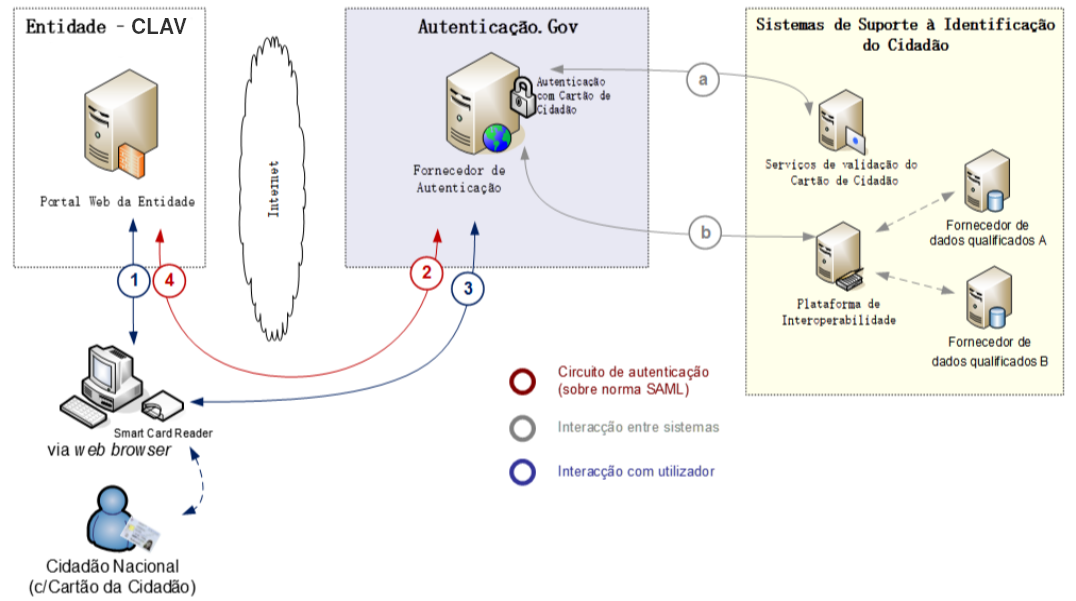
\includegraphics[width=1\textwidth]{img/fluxoauthgov.png}
    \end{center}
    \caption{Fluxo de pedidos entre a \acrshort{clav} e o Autenticação.gov de forma a autenticar um utilizador na \acrshort{clav}. Fonte:~\cite{agov}}\label{fig:fluxoauthgov}
\end{figure}

\begin{enumerate}
    \item O utilizador pretende aceder à área privada do portal de uma entidade (da \acrshort{clav}), na qual é necessário que comprove a sua identidade;
    \item O portal da entidade (\acrshort{clav}) delega a autenticação e redireciona o utilizador para o Autenticação.gov, juntamente com um pedido de autenticação assinado digitalmente;
    \item O Autenticação.gov valida o pedido de autenticação recebido e solicita a autenticação do utilizador com recurso ao seu \acrshort{cc} pedindo a inserção do seu \acrshort{pin} de autenticação. Durante este processo, o Autenticação.gov efetua as seguintes operações internas:
    \begin{enumerate}
        \item Valida as credenciais do utilizador com recurso à \acrshort{pki} do \acrshort{cc} via \acrshort{ocsp}
        \item Obtém atributos que sejam solicitados pelo portal da entidade (\acrshort{clav}) junto dos vários fornecedores de atributos qualificados. Esta operação é efetuada via Plataforma de Interoperabilidade. Este processo pode incluir a obtenção de dados da Federação de Identidades ou de outras Entidades.
    \end{enumerate}
    \item A identificação e atributos do utilizador são autenticadas e assinados digitalmente pelo Autenticação.gov, após o que redireciona o utilizador de volta ao portal da entidade original (\acrshort{clav}). Cabe à entidade (\acrshort{clav}) a validação das credenciais do Autenticação.gov e utilização dos atributos do cidadão.
\end{enumerate}

A troca de pedidos entre a \acrshort{clav} e o Autenticação.gov é feita através de \acrshort{saml} 2.0 (com as extensões que a \acrshort{ama} considera obrigatórias). De seguida será feita uma pequena introdução ao \acrshort{saml} 2.0. 

\subsection{\acrshort{saml} 2.0}
O \acrfull{saml} define uma \textit{framework} \textit{standard} em \acrshort{xml}.~\cite{sam2man} Foi aprovado pela \acrshort{oasis} e permite a troca segura de informação de autenticação e autorização entre diferentes entidades. Através do \acrshort{saml} é possível através de uma credencial (\textit{login} de um utilizador) aceder autenticado a um conjunto de \textit{websites}. Esta funcionalidade é conhecida por \acrfull{sso}.

Existem três tipos de papéis em \acrshort{saml}:~\cite{wisaml}
\begin{itemize}[leftmargin=2cm]
    \item Utilizador
    \item \textit{Identity Provider}: Realiza a autenticação de que o utilizador é quem diz ser e envia essa informação ao \textit{Service Provider} junta com as permissões de acesso do utilizador para o serviço
    \item \textit{Service Provider}: Precisa de autenticação do \textit{Identity Provider} para poder dar autorização ao utilizador
\end{itemize}

O documento \acrshort{xml} enviado pelo \textit{Identity Provider} para o \textit{Service Provider} é conhecida por \textit{\acrshort{saml} Assertion}. Existem três tipos de \textit{\acrshort{saml} Assertion}:~\cite{wisaml}
\begin{itemize}[leftmargin=2cm]
    \item \textit{Authentication Assertion}: Prova a identificação de um utilizador e fornece a hora em que o utilizador se autenticou e o método de autenticação usado
    \item \textit{Attribution Assertion}: Envia \textit{\acrshort{saml} attributes} (formato de dados que contém informação acerca do utilizador) para o \textit{Service Provider}
    \item \textit{Authorization Assertion}: Indica se o utilizador está autorizado a usar o serviço ou se o \textit{Identity Provider} recusou o pedido à inserção de uma password errada ou por falta de permissões para usar o serviço
\end{itemize}

No projeto \acrshort{clav} o utilizador final é o utilizador da \acrshort{clav}, o \textit{Identity Provider} é representado pelo Autenticação.gov e o \textit{Service Provider} é representado pela \acrshort{clav}.

%TODO
%\section{exceljs}
    %procurar "semelhantes" para cada um

%TODO
%\section{MongoDB}
%~\cite{wdmongo}

%TODO
%\section{mongoose}
%procurar "semelhantes" para cada um

%TODO
%\section{Web Semântica}
%~\cite{lsparql}

%TODO
%\subsection{RDF}
%~\cite{lsparql}

%TODO
%\subsection{SPARQL}
%~\cite{lsparql}

%TODO
%se calhar referir algumas packages de ligação ao sparql em vez de usar o que criei

%TODO
%\section{GraphDB}
%procurar "semelhantes" para cada um (Neo4j)

\section{Swagger}
O \textit{Swagger} é um ecossistema de ferramentas para desenvolver \acrshort{api}s com a \acrfull{oas}.

Até 2015 o \textit{Swagger} consistia numa especificação e num ecossistema de ferramentas para implementar a especificação. Em 2015 a fundadora do \textit{Swagger}, \textit{SmartBear Software}, doou a especificação \textit{Swagger} para a \textit{Linux Foundation} e renomeou a especificação para \acrlong{oas}.~\cite{wiswagger}

A especificação \textit{OpenAPI} é agora desenvolvida pela \textit{OpenAPI Initiative} que envolve várias empresas tecnológicas entre as quais \textit{Microsoft}, \textit{Google}, \textit{IBM} e a fundadora \textit{Smartbear Software}.

Já o conjunto de ferramentas \textit{Swagger} inclui ferramentas \textit{open-source}, gratuitas e comerciais que podem ser usadas em diferentes estágios do ciclo de vida de uma \acrshort{api}, que inclui documentação, desenho, testes e \textit{deployment}. Algumas das ferramentas são:~\cite{swaggerVSoas}
\begin{itemize}
    \item \textbf{\textit{Swagger Editor}}: Permite editar especificações \textit{OpenAPI} em \acrshort{yaml} no \textit{browser}\footnote{Aceder \url{https://editor.swagger.io/}}, validar as especificações em relação às regras do \acrshort{oas} bem como pré-visualizar a documentação em tempo real. Facilita o desenho e a documentação de \acrshort{api}s \acrshort{rest}
    \item \textbf{\textit{Swagger \acrshort{ui}}}: Coleção de \textit{assets} \textit{\acrshort{html}}, \textit{JavaScript} e \textit{\acrshort{css}} que geram dinamicamente documentação a partir de uma especificação \textit{OpenAPI} de uma \acrshort{api}
    \item \textbf{\textit{Swagger Codegen}}: Permite a geração de bibliotecas cliente (geração de \acrshort{sdk}), \textit{server stubs} e documentação automática a partir de especificações \textit{OpenAPI}
    \item \textbf{\textit{Swagger Inspector}} (gratuita): Ferramenta de testes de \acrshort{api}s que permite validar as \acrshort{api}s e gerar definições \textit{OpenAPI} de \acrshort{api}s existentes
    \item \textbf{\textit{SwaggerHub}} (gratuita e comercial): Desenho e documentação de \acrshort{api}s, construído para equipas que trabalham com \textit{OpenAPI}
\end{itemize}

O \textit{Swagger} possui duas abordagens:~\cite{swaggerNode}
\begin{itemize}
    \item \textit{top-down}: Uso do \textit{Swagger Editor} para criar a especificação \textit{OpenAPI} e depois usar o \textit{Swagger Codegen} por forma a gerar o código do cliente e do servidor. Ou seja, primeiro desenha-se a \acrshort{api} antes de escrever código
    \item \textit{bottom-up}: Utilizador já possui uma \acrshort{api} \acrshort{rest} e o \textit{Swagger} irá ser usado apenas para documentar a \acrshort{api} existente
\end{itemize}

Visto que a \acrshort{clav} já possui grande parte da \acrshort{api} construída vai ser usada uma abordagem \textit{bottom-up}. Portanto, o \textit{Swagger} vai ser usado apenas para a documentação da \acrshort{api}. De forma a produzir a documentação, do portfólio de ferramentas do \textit{Swagger} apenas precisaremos de utilizar o \textit{Swagger \acrshort{ui}} e o \textit{Swagger Editor}. O primeiro permitirá apresentar aos utilizadores a documentação gerada e o segundo permitirá validar a especificação \textit{OpenAPI} (documentação) criada, verificando se não possui erros.

\subsection{Especificação \textit{OpenAPI}}

A especificação \textit{OpenAPI} providencia um conjunto de propriedades que podem ser usadas para descrever uma \acrshort{api} \acrshort{rest}. Com um documento de especificação válido é possível usá-lo para criar uma documentação interativa, por exemplo, através do \textit{Swagger \acrshort{ui}}.

De seguida será apresentado o que é possível documentar com a especificação \textit{OpenAPI} e como. É possível usar \acrshort{yaml} como \acrshort{json} para a especificar. Esta parte será demonstrada usando \acrshort{yaml}.\footnote{A especificação completa do \textit{OpenAPI} com versão igual a 3.0.0 pode ser vista em \url{https://github.com/OAI/OpenAPI-Specification/blob/master/versions/3.0.0.md}}

\subsubsection{Metadata}
O primeiro passo é escolher a versão da especificação \textit{OpenAPI} que irá ser usada para documentar:
\begin{lstlisting}[language=yaml, caption=Exemplo de indicação da versão da especificação \textit{OpenAPI}]
openapi: 3.0.0
\end{lstlisting}

Depois na secção \texttt{info} é possível descrever um pouco sobre a \acrshort{api} que estamos a documentar, indicando o título, a descrição e a versão da \acrshort{api}. As propriedades \texttt{title} e \texttt{version} são obrigatórias. É possível também colocar informação sobre os contactos disponíveis, termos de uso e a licença:\footnote{Ver mais em \url{https://github.com/OAI/OpenAPI-Specification/blob/master/versions/3.0.0.md\#infoObject}}
\begin{lstlisting}[language=yaml, caption={Exemplo de secção \texttt{info} indicando título, descrição e versão da \acrshort{api} na especificação \textit{OpenAPI}}]
info:
  title: CLAV API
  description: Esta é a API do projeto CLAV...
  version: 1.0.0
\end{lstlisting}

\vspace{-0.7cm}

\subsubsection{Servidores}
Há depois uma secção com o nome de \texttt{servers} para indicar os \textit{URL}s da \acrshort{api} que se pode aceder. Podem ser indicados mais do que um \textit{URL}:\footnote{Para mais detalhes sobre esta secção veja \url{https://swagger.io/docs/specification/api-host-and-base-path/}}
\begin{lstlisting}[language=yaml, caption=Exemplo de secção \texttt{servers} indicando os \textit{URL}s e a descrição de cada na especificação \textit{OpenAPI}]
servers:
  - url: http://clav-api.dglab.gov.pt/api
    description: Official API server
  - url: http://clav-test.di.uminho.pt/api
    description: Testing server
  - url: http://localhost:7779/api
    description: Local server
\end{lstlisting}

\vspace{-0.7cm}

\subsubsection{Caminhos/Rotas}
De seguida apresenta-se uma das secções mais importantes da especificação, a secção \texttt{paths}. Aqui são definidas as rotas que a \acrshort{api} disponibiliza. Para definir cada rota basta indicar o caminho relativo aos \acrshort{url}s definidos na secção \texttt{servers} (\verb|<server-url>/<caminho relativo>|). Nesta secção é definido tudo que envolve as rotas, desde os parâmetros necessários, as respostas que devolve, os métodos \textit{HTTP} disponíveis, etc:\footnote{Mais detalhes em \url{https://swagger.io/docs/specification/paths-and-operations/}}\footnote{mais detalhes sobre a funcionalidade \texttt{\$ref} em \url{https://swagger.io/docs/specification/using-ref/}}
\begin{lstlisting}[language=yaml, caption=Exemplo de secção \texttt{paths} indicando os detalhes de cada rota na especificação \textit{OpenAPI}, label={exem:oapiRota}]
paths:
  /users/{id}:
    get:
      summary: Resumo do que faz a rota
      description: >
        Descrição detalhada, pode ser usado Markdown para enriquecer o texto
      parameters:
        - name: id
          in: path
          description: Id do utilizador
          required: true
          schema:
            type: string
      responses:
        200:
          description: Descrição da resposta, p.e: Sucesso
          content:
            application/json:
              schema:
                #A estrutura do JSON devolvido pode ser definido logo aqui ou num componente à parte, fazendo referência desse. Iremos aplicar o segundo caso para demonstrar que estas funcionalidades tornam a documentação mais fácil de manter
                $ref: '#/components/schemas/User'
    post:
      ...
    delete:
      ...
  /users:
    ...

components:
  schemas:
    User:
      type: object
      properties:
        id:
          type: string
        ...
      required:
        - id
        ...
\end{lstlisting}

Outro ponto importante a referir é que é possível agrupar as rotas em grupos através do uso de \textit{tags}. As \textit{tags} tem de ser definidas numa secção chamada \textit{tags}:
\begin{lstlisting}[language=yaml, caption={Exemplo de secção \texttt{tags} defininfo tags na especificação \textit{OpenAPI}}]
tags:
  - name: users
    description: Descrição
  - name: classes
    description: Outra descrição
\end{lstlisting}

Depois em cada rota é necessário indicar a que \textit{tag} (grupo) pertence:
\begin{lstlisting}[language=yaml, caption=Exemplo de uso de \textit{tags} numa rota na especificação \textit{OpenAPI}]
paths:
  /users/{id}:
    get:
      summary: Resumo do que faz a rota
      tags:
        - users
      ...
\end{lstlisting}

\vspace{-0.7cm}

\subsubsection{Parâmetros}\label{sec:paramSwagger}
Como já exemplificado no exemplo~\ref{exem:oapiRota} os parâmetros de uma rota são definidos na secção \texttt{parameters} de cada rota. Existem quatro tipo de parâmetros que variam de acordo com o local onde se encontram. O tipo de um parâmetro é definido na propriedade \texttt{in} de um parâmetro e pode ser um dos seguintes:
\begin{itemize}
    \item Parâmetros no caminho: Servem normalmente para apontar para um recurso específico. Estes parâmetros são sempre obrigatórios como tal a propriedade \texttt{required} com o valor igual a verdadeiro deve ser sempre adicionado. Para além disso o \texttt{name} tem de ser igual ao que está no caminho. A propriedade \texttt{in} tem o valor de \textit{path}.
    \item Parâmetros na \textit{query string}: A propriedade \texttt{in} tem o valor de \textit{query}. No caso de tokens passados em parâmetros da \textit{query string} deve-se usar esquemas de segurança, veja a secção~\ref{sec:authSwagger} Autenticação.
    \item Parâmetros no cabeçalho: A propriedade \texttt{in} tem o valor de \textit{header}. Contudo os cabeçalhos \textit{Accept}, \textit{Content-Type} e \textit{Authorization} não são aqui definidos.
    \item Parâmetros no cabeçalho da \textit{Cookie}: A propriedade \texttt{in} tem o valor de \textit{cookie}.
\end{itemize}

Cada parâmetro tem várias propriedades que permitem defini-lo:\footnote{Mais detalhes em \url{https://swagger.io/docs/specification/describing-parameters/}}
\begin{itemize}
    \item \texttt{required}: Indica se o parâmetro é obrigatório ou opcional. Possíveis valores são \textit{true} ou \textit{false}.
    \item Na propriedade \texttt{schema}:
    \begin{itemize}
        \item \texttt{default}: Valor padrão de um parâmetro opcional
        \item \texttt{type}: O tipo do parâmetro. Possíveis valores: \textit{string}, \textit{integer}, etc
        \item \texttt{enum}: Indica os possíveis valores para o parâmetro
        \item \texttt{nullable}: Indica se o parâmetro pode ser \textit{null}. Possíveis valores são \textit{true} ou \textit{false}.
    \end{itemize}
    \item \texttt{allowEmptyValue}: Indica se o parâmetro pode ser vazio. Apenas aplicável no caso de um parâmetro na \textit{query string}. Possíveis valores são \textit{true} ou \textit{false}.
    \item \texttt{example}: Um exemplo do valor
    \item \texttt{examples}: Múltiplos exemplos
    \item \texttt{deprecated}: Indica se o parâmetro é ou não \textit{deprecated}. Possíveis valores são \textit{true} ou \textit{false}.
\end{itemize}

\subsubsection{\textit{Request Body}}
O \textit{request body} é definido em cada rota na secção \texttt{requestBody} sendo usado essencialmente em rotas com o método \acrshort{http} igual a POST ou a PUT, ou seja, em casos que há necessidade de criar ou alterar um objeto de acordo com a informação fornecida no pedido. As propriedades que podem ser definidas no \texttt{requestBody} são as seguintes:\footnote{Para mais detalhes, desde \textit{upload} de ficheiros, a \textit{Form Data}s, veja em \url{https://swagger.io/docs/specification/describing-request-body/}}\footnote{Para mais informação sobre os \textit{media types} veja \url{https://swagger.io/docs/specification/media-types/}}
\begin{itemize}
    \item \texttt{description}: Opcionalmente pode ser adicionada uma descrição
    \item \texttt{required}: Indica se o \textit{request body} é obrigatório ou opcional. Possíveis valores são \textit{true} ou \textit{false}. Por padrão o \textit{request body} é opcional.
    \item \texttt{content}: Obrigatório. Lista os \textit{media types} consumidos pela rota e especifica o \texttt{schema} para cada \textit{media type}
\end{itemize}

\subsubsection{Respostas}
Nesta secção, propriedade \texttt{responses} de cada rota, é descrita as possíveis respostas de cada rota. Na propriedade será definido as várias respostas, uma resposta por cada \acrshort{http} \textit{status code} possível de ser devolvido pela rota. Cada resposta pode possuir as seguintes propriedades:\footnote{Mais detalhes em \url{https://swagger.io/docs/specification/describing-responses/}}
\begin{itemize}
    \item \texttt{description}: Obrigatório, descrição da resposta
    \item \texttt{content}: Opcional, semelhante ao \texttt{content} do \textit{request body} e define o conteúdo que é devolvido.
    \item \texttt{headers}: Opcional, define as \textit{headers} que são devolvidas na resposta
\end{itemize}

\subsubsection{Adição de Exemplos}
Na secção~\ref{sec:paramSwagger} Parâmetros já se referiu como é possível adicionar exemplos aos parâmetros. De forma semelhante o mesmo pode ser realizado tanto no \textit{request body} como nas respostas através da propriedade \texttt{example} (um exemplo) ou \texttt{examples} (múltiplos exemplos) aninhado na propriedade \texttt{schema} ou aninhado na ``propriedade'' \textit{media type} no caso do \texttt{schema} ser uma referência para um modelo presente na secção \texttt{components}. A propriedade \texttt{example} pode também ser usada em objetos ou propriedades de um \texttt{schema}. Por fim, para adicionar exemplos de \acrshort{xml} ou \acrshort{html} os exemplos devem ser exemplificados como \textit{strings}:\footnote{Mais detalhes em \url{https://swagger.io/docs/specification/adding-examples/}}
\begin{lstlisting}[language=yaml, caption=Exemplo de adição de exemplos para \acrshort{xml} e \acrshort{html} na especificação \textit{OpenAPI}]
content:
  application/xml:
    schema:
      $ref: '#/components/schemas/xml'
    examples:
      xml:
        summary: A sample XML response
        value: '<objects><object><id>1</id><name>new</name></object><object><id>2</id></object></objects>'
  text/html:
    schema:
      type: string
      examples:
        html:
          summary: A list containing two items
          value: '<html><body><ul><li>item 1</li><li>item 2</li></ul></body></html>'
\end{lstlisting}

\subsubsection{Modelos}
A secção \texttt{schemas} presente na secção \texttt{components} permite definir estruturas de dados (modelo) a serem usados na \acrshort{api}. Estes modelos podem ser referenciados usando a funcionalidade \texttt{\$ref}.\footnote{Mais detalhes em \url{https://swagger.io/docs/specification/data-models/}}

\subsubsection{Autenticação e Autorização}\label{sec:authSwagger}
Nesta secção será demonstrada como se pode adicionar a autenticação e autorização à especificação \textit{OpenAPI}. Para tal é necessário criar \textit{security scheme}s. Os esquemas são definidos na secção \texttt{securitySchemes} dentro da secção \texttt{components}. Para cada esquema de segurança é necessário definir a propriedade \texttt{type}. Na especificação é possível descrever os seguintes esquemas de segurança:
\begin{itemize}
    \item Esquemas de autenticação \acrshort{http} (usam o cabeçalho \textit{Authorization}) (\texttt{type} = \texttt{http}):
    \begin{itemize}
        \item \textit{Basic} (propriedade \texttt{scheme} = \texttt{basic})
        \item \textit{Bearer} (propriedade \texttt{scheme} = \texttt{bearer} e pode também ser definido o formato do \textit{Bearer} (a palavra usada antes de indicar o \textit{token}) através da propriedade \texttt{bearerFormat})
        \item Outros esquemas \acrshort{http} definidos pelo \href{https://tools.ietf.org/html/rfc7235}{RFC 7235} e pelo registo de esquemas de autenticação \acrshort{http}
    \end{itemize}
    \item Chaves \acrshort{api} no cabeçalho, na \textit{query string} ou em \textit{cookies} (\texttt{type} = \texttt{apiKey} e na propriedade \texttt{in} indicar em que local se encontra, se no cabeçalho (\texttt{header}), se na \textit{query string} (\texttt{query}) ou se nas \textit{cookies} (\texttt{cookie}))
    \item \textit{OAuth 2} (\texttt{type} = \texttt{oauth2})
    \item \textit{OpenID Connect Discovery} (\texttt{type} = \texttt{openIdConnect})
\end{itemize}

Após definir os esquemas de segurança é necessário aplicá-los nas rotas que devem estar protegidas por esses esquemas. Para tal em cada rota pode ser definida a propriedade \texttt{security} e indicar os esquemas de segurança que essa rota suporta.\footnote{Mais detalhes em \url{https://swagger.io/docs/specification/authentication/}}

\subsubsection{Alternativas}
Em termos de alternativas à especificação \textit{OpenAPI} existem duas concorrentes: \textit{\acrshort{raml}}\footnote{Ver \url{https://github.com/raml-org/raml-spec/blob/master/versions/raml-10/raml-10.md/}} e \textit{\acrshort{api} Blueprint}\footnote{Ver \url{https://github.com/apiaryio/api-blueprint/blob/master/API\%20Blueprint\%20Specification.md}}.

Comparemos as três hipóteses:~\cite{specsComp}
\begin{table}[H]
    \footnotesize
    \begin{center}
    \begin{tabular}{|r|p{0.385\textwidth}|p{0.385\textwidth}|}
    \hline
    Especificação & Vantagens & Desvantagens \\ \hline
    \textit{OpenAPI} &
        \begin{itemize}[leftmargin=0.3cm]
            \setlength\itemsep{0em}
            \item Grande adoção
            \item Grande comunidade de utilizadores
            \item Bom suporte
            \item Suporte para várias linguagens
        \end{itemize}
        &
        \begin{itemize}[leftmargin=0.3cm]
            \setlength\itemsep{0em}
            \item Falta de construtores avançados para metadados
        \end{itemize}
        \\ \hline
    \acrshort{raml} &
        \begin{itemize}[leftmargin=0.3cm]
            \setlength\itemsep{0em}
            \item Suporta construções avançadas
            \item Adoção decente
            \item \textit{Human readable format}
            \item Grande apoio da indústria 
        \end{itemize}
        &
        \begin{itemize}[leftmargin=0.3cm]
            \setlength\itemsep{0em}
            \item Falta de ferramentas ao nível do código
            \item Ainda não comprovado a longo prazo
        \end{itemize}
        \\ \hline
    \textit{\acrshort{api} Blueprint} &
        \begin{itemize}[leftmargin=0.3cm]
            \setlength\itemsep{0em}
            \item Fácil de entender
            \item Simples de escrever
        \end{itemize}
        &
        \begin{itemize}[leftmargin=0.3cm]
            \setlength\itemsep{0em}
            \item Pouca adoção
            \item Falta de construtores avançados
            \item Instalação complexa
        \end{itemize}
        \\ \hline
    \end{tabular}
    \end{center}
    \caption{Comparação entre especificações de documentação de \acrshort{api}s}
\end{table}

Além das vantagens apresentadas as três são \textit{open-source}. Para além disso, o \textit{OpenAPI} pode ser escrito em \acrshort{json} ou \acrshort{yaml}, o \acrshort{raml} é escrito em \acrshort{yaml} e o \textit{\acrshort{api} Blueprint} é escrito em \textit{Markdown}. Escolheu-se a especificação \textit{OpenAPI} devido à sua grande adoção e por permitir usar o ecossistema de ferramentas \textit{Swagger}.

\subsection{\textit{Swagger \acrshort{ui}}}

O \textit{Swagger \acrshort{ui}} permite a qualquer um visualizar uma \acrshort{api} \acrshort{rest}. A partir de um documento \acrshort{json} ou \acrshort{yaml} (especificação \textit{OpenAPI}) é automaticamente gerado uma documentação interativa.

\begin{figure}[H]
    \begin{center}
        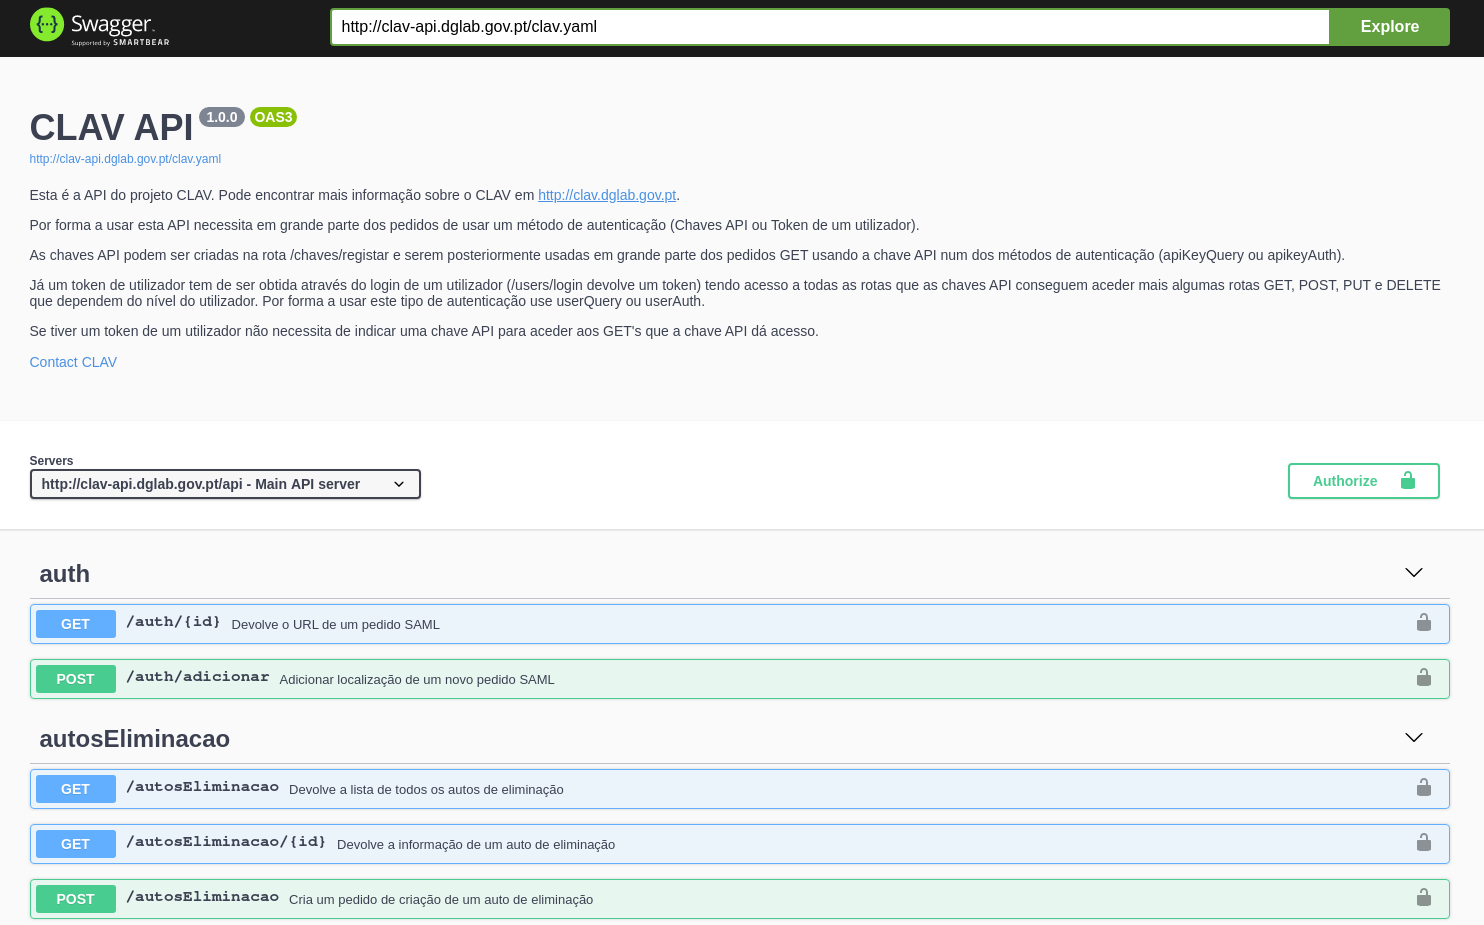
\includegraphics[width=0.5\textwidth]{img/swaggerUI.png}
    \end{center}
    \caption{\textit{Swagger \acrshort{ui}} exemplo}
\end{figure}

\subsubsection{Alternativas}
Existem várias alternativas ao \textit{Swagger \acrshort{ui}}:
\begin{savenotes}
\begin{table}[H]
    \footnotesize
    \begin{center}
    \begin{tabular}{|r|p{0.39\textwidth}|p{0.39\textwidth}|}
    \hline
    Ferramenta & Vantagens & Desvantagens \\ \hline
        \textit{Swagger \acrshort{ui}} &
        \begin{itemize}[leftmargin=0.3cm]
            \setlength\itemsep{0em}
            \item Suporta a especificação \textit{OpenAPI}
            \item \textit{Open-source}
            \item Amplamente usado
        \end{itemize}
        &
        %\begin{itemize}[leftmargin=0.3cm]
        %    \setlength\itemsep{0em}
        %    \item
        %\end{itemize}
        \\ \hline
    \textit{Apiary}\footnote{Ver \url{https://apiary.io/}} &
        \begin{itemize}[leftmargin=0.3cm]
            \setlength\itemsep{0em}
            \item Suporta a especificação \textit{\acrshort{api} Blueprint} e a especificação \textit{OpenAPI}
        \end{itemize}
        &
        \begin{itemize}[leftmargin=0.3cm]
            \setlength\itemsep{0em}
            \item Necessário pagar de forma a puder integrar a documentação da \acrshort{api} num domínio próprio
            \item \textit{Closed-source}
        \end{itemize}
        \\ \hline
    \textit{\acrshort{api} Console}\footnote{Ver \url{https://github.com/mulesoft/api-console}} &
        \begin{itemize}[leftmargin=0.3cm]
            \setlength\itemsep{0em}
            \item Suporta a especificação \acrshort{raml} e a especificação \textit{OpenAPI}
            \item \textit{Open-source}
        \end{itemize}
        &
        %\begin{itemize}[leftmargin=0.3cm]
        %    \setlength\itemsep{0em}
        %    \item
        %\end{itemize}
        \\ \hline
    \textit{Slate}\footnote{Ver \url{https://github.com/slatedocs/slate}} &
        \begin{itemize}[leftmargin=0.3cm]
            \setlength\itemsep{0em}
            \item \textit{Open-source}
            \item \acrshort{api} definida em \textit{Markdown}
        \end{itemize}
        &
        \begin{itemize}[leftmargin=0.3cm]
            \setlength\itemsep{0em}
            \item Não suporta nenhuma especificação
        \end{itemize}
        \\ \hline
    \textit{apiDoc}\footnote{Ver \url{https://apidocjs.com/}} &
        \begin{itemize}[leftmargin=0.3cm]
            \setlength\itemsep{0em}
            \item Documentação criada a partir das anotações nos comentários do código
            \item \textit{Open-source} 
        \end{itemize}
        &
        \begin{itemize}[leftmargin=0.3cm]
            \setlength\itemsep{0em}
            \item Não suporta nenhuma especificação
        \end{itemize}
        \\ \hline
    \textit{ReDoc}\footnote{Ver \url{https://github.com/Redocly/redoc}} &
        \begin{itemize}[leftmargin=0.3cm]
            \setlength\itemsep{0em}
            \item Suporta a especificação \textit{OpenAPI}
            \item \textit{Open-source} 
            \item Fácil de integrar
        \end{itemize}
        &
        %\begin{itemize}[leftmargin=0.3cm]
        %    \setlength\itemsep{0em}
        %    \item
        %\end{itemize}
        \\ \hline
    \end{tabular}
    \end{center}
    \caption{Comparação entre ferramentas de \acrshort{api}s}
\end{table}
\end{savenotes}

De forma a escolher a ferramenta apropriada é necessário ter em conta que:
\begin{itemize}
    \item Não há financiamento
    \item Já existe uma \acrshort{api} desenvolvida
    \item A documentação deve estar acessível de um domínio próprio
    \item A documentação deve ser fácil de criar, de editar e de manter
    \item Será usada a especificação \textit{OpenAPI}
\end{itemize}

As escolhas ficam como tal reduzidas ao \textit{Swagger \acrshort{ui}} e ao \textit{ReDoc}. Optou-se por escolher o \textit{Swagger \acrshort{ui}} visto ser a ferramenta mais amplamente usada para além de que é possível obter também uma fácil integração no \textit{Swagger \acrshort{ui}} com recurso à package \texttt{swagger-ui-express} que falaremos na próxima secção.

\section{Documentação da \acrshort{api} do \acrshort{clav}}

Agora sabendo que será usada a especificação \textit{OpenAPI} e o \textit{Swagger \acrshort{ui}} é importante perceber que bibliotecas devem ser usadas para a produção da documentação. 

Existem duas \textit{packages} que podem ser usadas para criar documentação interativa para uma \acrshort{api} \acrshort{rest} criada com \textit{Node.js} e \textit{Express.js}:~\cite{swaggerNode}
\begin{itemize}
    \item \texttt{swagger-node-express}
    \begin{itemize}
        \item Vantagens
        \begin{itemize}
            \item Módulo oficial suportado pelo \textit{Swagger}
            \item É \textit{open-source} e como tal é possível contribuir para a correção de problemas
            \item A solução contém \textit{Swagger Editor} e \textit{Swagger Codegen} e como tal tanto podemos usar uma abordagem \textit{top-down} como \textit{bottom-up}
        \end{itemize}
        \item Desvantagens
        \begin{itemize}
            \item Instalação manual do \textit{Swagger \acrshort{ui}}. O código do \textit{Swagger \acrshort{ui}} tem de ser copiado manualmente para o projeto e sempre que há uma atualização é necessário copiar novamente manualmente
            \item Instalação complexa. Por forma a aplicação hospedar a documentação é necessário adicionar algumas rotas ao servidor para além das já definidas na especificação \textit{OpenAPI}
            \item Fraca documentação
        \end{itemize}
    \end{itemize}
    \item \texttt{swagger-ui-express}
    \begin{itemize}
        \item Vantagens
        \begin{itemize}
            \item É \textit{open-source} e como tal é possível contribuir para a correção de problemas
            \item Não é necessário copiar manualmente o \textit{Swagger \acrshort{ui}}
            \item De fácil instalação, apenas é necessário adicionar uma rota aonde estará hospedada a documentação
            \item Boa documentação
        \end{itemize}
        \item Desvantagens
        \begin{itemize}
            \item Não é o módulo oficial suportado pelo \textit{Swagger}
        \end{itemize}
    \end{itemize}
\end{itemize}

Das duas foi escolhida a \texttt{swagger-ui-express} visto ser de mais simples implementação e de mais fácil manutenção.

\begin{lstlisting}[language=javascript, caption=Exemplo de uso do \texttt{swagger-ui-express}, label=exem:suie]
var swaggerUI = require('swagger-ui-express')
//JSON
var swaggerDocument = require('./swagger.json')
//ou YAML
var yaml = require('js-yaml')
var fs = require('fs')
var swaggerDocument = yaml.load(fs.readFileSync('./swagger.yaml'))

app.use('/doc', swaggerUI.serve, swaggerUI.setup(swaggerDocument));
\end{lstlisting}

No exemplo~\ref{exem:suie} a documentação da \acrshort{api} está presente na rota \texttt{'/doc'}. Neste exemplo é exemplificado como carregar uma especificação \textit{OpenAPI} em \acrshort{json} bem como em \acrshort{yaml}. Quanto ao \textit{middleware} \texttt{serve} retorna os ficheiros estáticos necessários para hospedar o \textit{Swagger \acrshort{ui}}. Já o segundo \textit{middleware} \texttt{setup} para além de puder receber o documento com a especificação \textit{OpenAPI} pode também receber um outro parâmetro de opções que o utilizador pode definir para a apresentação interativa da documentação com o \textit{Swagger \acrshort{ui}}\footnote{As opções possíveis estão presentes em \url{https://github.com/scottie1984/swagger-ui-express}. Para o atributo (opção) \texttt{swaggerOptions} as opções possíveis estão presentes em \url{https://github.com/swagger-api/swagger-ui/blob/master/docs/usage/configuration.md}}.

Agora há duas abordagens possíveis de realizar a documentação:
\begin{itemize}
    \item Documentação de cada rota nos comentários da rota através da utilização da \textit{package} \texttt{swagger-jsdoc}\footnote{Ver \url{https://github.com/Surnet/swagger-jsdoc}}
    \item Documentação à parte do código
\end{itemize}

A abordagem escolhida foi a da documentação à parte do código por forma a modularizar a documentação. A modularização da documentação foi realizada através do uso da \textit{package} \texttt{yaml-include}\footnote{Ver \url{https://github.com/claylo/yaml-include}}. Esta \textit{package} permite que o documento \acrshort{yaml} da especificação \textit{OpenAPI} possa ser dividida por vários ficheiros. Ela permite a inclusão de arquivos \acrshort{yaml} externos ou a inclusão de pastas de ficheiros \acrshort{yaml}. Esta funcionalidade é desaprovada pela equipa de desenvolvimento do \acrshort{yaml} contudo é de grande ajuda e de simplificação da construção do ficheiro de especificação \textit{OpenAPI}.

\begin{lstlisting}[language=yaml, caption=Exemplo de uso do \texttt{yaml-include} no documento de especificação \textit{OpenAPI}(\textit{index.yaml}), label=exem:yamli]
openapi: 3.0.0
info:
  description: Esta é a API do projeto CLAV. Pode encontrar mais informação sobre o CLAV em [http://clav.dglab.gov.pt](http://clav.dglab.gov.pt).
  version: 1.0.0
  title: CLAV API
  contact:
    name: CLAV
    email: clav@dglab.gov.pt
servers:
  - url: http://localhost:7779/api
    description: Local API server
paths: !!inc/dir [ 'paths' ]
components:
  schemas: !!inc/dir [ 'schemas', excludeTopLevelDirSeparator: true ]
\end{lstlisting}

O ficheiro \textit{index.yaml} será a raiz do documento de especificação \textit{OpenAPI} a ser gerado com a \textit{package} \texttt{yaml-include}. A estrutura dos ficheiros para gerar o documento de especificação \textit{OpenAPI} final exemplifica como se pode dividir a documentação por vários ficheiros com esta \textit{package}:
\begin{lstlisting}[language=pseudocode, caption=Exemplo de estrutura dos ficheiros para gerar o documento de especificação \textit{OpenAPI}, label=exem:faf]
* index.yaml
* paths/
    * classes/
        * get.yaml
        * ~id/
            * get.yaml
    * users/
        * ~id/
            * post.yaml
            * delete.yaml
* schemas/
    * User.yaml
\end{lstlisting}

Assim, o \texttt{!!inc/dir} fará que no ficheiro \textit{index.yaml} na \textit{tag} \textit{paths} sejam incluídos todos os ficheiros que estão na pasta \textit{paths}. Cada ficheiro corresponderá a uma determinada rota com um determinado método \acrshort{http}. O método \acrshort{http} é definido a partir do nome do ficheiro e o caminho da rota é determinado pelo nome das pastas e do aninhamento destas. Quando o nome da pasta é iniciado por ``\verb|~|'' no caminho será colocado o nome da pasta sem o til entre chavetas (``\{\}'') por forma a indicar um parâmetro que é colocado no caminho do pedido.

Já no caso do \texttt{!!inc/dir} dos \textit{schemas} a opção \texttt{excludeTopLevelDirSeparator} permite que os ficheiros que estejam dentro da pasta \textit{schemas} (mas não aninhados dentro de outras pastas) sejam incluídos sem qualquer aninhamento, assumindo o nome do ficheiro como o atributo a colocar.

O documento de especificação \textit{OpenAPI} final gerado será:
\begin{lstlisting}[language=yaml, caption=Documento de especificação \textit{OpenAPI} gerado a partir do ficheiro \textit{index.yaml} com o uso da \textit{package} \texttt{yaml-include}, label=exem:yamlif]
openapi: 3.0.0
info:
  description: Esta é a API do projeto CLAV. Pode encontrar mais informação sobre o CLAV em [http://clav.dglab.gov.pt](http://clav.dglab.gov.pt).
  version: 1.0.0
  title: CLAV API
  contact:
    name: CLAV
    email: clav@dglab.gov.pt
servers:
  - url: http://localhost:7779/api
    description: Local API server
paths:
  /classes:
    get:
      <conteúdo do ficheiro paths/classes/get.yaml>
  /users/{id}:
    post:
      <conteúdo do ficheiro paths/~id/post.yaml>
    delete:
      <conteúdo do ficheiro paths/~id/delete.yaml>
components:
  schemas:
    User:
      <conteúdo do ficheiro schemas/User.yaml>
\end{lstlisting}

No final teremos um ficheiro no formato \acrshort{yaml} com toda a documentação da \acrshort{api} que puderá então ser usado para alimentar a documentação dinâmica \textit{Swagger \acrshort{ui}}.

%TODO
%\section{Importação de dados}
%TODO: falar da tabela de seleção

\section{Exportação de dados}
Um dos requisitos da \acrshort{api} da \acrshort{clav} é permitir a exportação de Classes, Entidades, Tipologias e Legislações em formato \acrshort{json}, \acrshort{xml} e \acrshort{csv}. Deve também permitir exportar toda a ontologia do projeto nos formatos \acrshort{turtle}, \acrshort{json-ld} e \acrshort{rdf}/\acrshort{xml}.

Para a primeira parte foi necessário desenvolver dois conversores, de \acrshort{json} para \acrshort{xml} e de \acrshort{json} para \acrshort{csv} visto que o \acrshort{json} já é por predefinição devolvido.

\subsection{\acrshort{xml}}
O conversor de \acrshort{json} para \acrshort{xml} criado é representado pelo algoritmo presente no anexo~\ref{exem:convXML}.

Com este algoritmo, os dados exportados estarão sempre encapsulados na \textit{tag} \texttt{root} por forma a garantir que só existe um elemento \textit{root} no documento \acrshort{xml} gerado respeitando as regras do \acrshort{xml}. Cada tipo de dados do \acrshort{json} é convertido da seguinte forma:
\begin{itemize}
    \item \textit{string}: Mantém-se igual tirando os caracteres ``\texttt{<}'', ``\texttt{>}'', ``\texttt{\&}'', ``\texttt{'}'' e ``\texttt{"}'' que são convertidos para a \textit{Entity Reference}\footnote{``\texttt{<}'' para ``\texttt{\&lt;}'', ``\texttt{>}'' para ``\texttt{\&gt;}'', ``\texttt{\&}'' para ``\texttt{\&amp;}'', ``\texttt{'}'' para ``\texttt{\&apos;}'' e ``\texttt{"}'' para ``\texttt{\&quot;}''} correspondente
    \item \textit{number}: Mantém-se igual
    \item \textit{boolean}: Mantém-se igual
    \item \textit{null}: Origina uma \textit{string} vazia
    \item \textit{array}: Cada item do \textit{array} é encapsulado numa \textit{tag} \texttt{item} que possui um atributo \texttt{index} que indica a posição do elemento no \textit{array} e um atributo \texttt{type} que indica o tipo do elemento do \textit{array}. O tipo pode ser \textit{number}, \textit{boolean}, \textit{string}, \textit{array} ou \textit{object}.
    \item \textit{object}: Para cada propriedade será criado uma \textit{tag} com valor igual à chave da propriedade e ao valor da propriedade será aplicado recursivamente uma das transformações desta lista. Esta \textit{tag} terá um atributo \texttt{type} em que o seu valor, tal como nos \textit{arrays}, pode ser \textit{number}, \textit{boolean}, \textit{string}, \textit{array} ou \textit{object}.
\end{itemize}

Apresenta-se no anexo~\ref{conv:jsonTOxml} uma conversão exemplo.

\subsection{\acrshort{csv}}

Da mesma forma que o \acrshort{xml}, o \acrshort{csv} é convertido sem recurso a uma biblioteca que converta já de si o \acrshort{json} para \acrshort{csv} visto que cada objeto \acrshort{json} a exportar necessita de uma exportação personalizada para \acrshort{csv}. Ao contrário do conversor desenvolvido para \acrshort{xml}, o conversor para \acrshort{csv} não converte qualquer objeto para \acrshort{csv} mas apenas um conjunto restrito de objetos \acrshort{json}.

O algoritmo de conversão de \acrshort{json} para \acrshort{csv} desenvolvido pode ser visualizado no anexo~\ref{exem:convCSV}.

O conjunto de objetos permitidos é lista de classes, de entidades, de tipologias e de legislações e objeto de classe, de entidade, de tipologia e de legislação.

Quanto à conversão em si, possui uma estrutura interna durante a conversão. Esta estrutura é uma lista de listas, em que cada lista representa uma linha do \acrshort{csv}. Cada elemento de uma das listas representará uma célula do \acrshort{csv}. A primeira lista será a primeira linha do \acrshort{csv} e como tal possuirá os títulos. As restantes listas serão as linhas seguintes do \acrshort{csv} em que cada elemento possuirá os valores já transformados em \textit{strings} dos campos dos objetos.

Para além desta estrutura interna existe um dicionário que permite agilizar o algoritmo de conversão. Este dicionário possuirá vários dicionários, um por cada objeto (Classe, Entidade, Tipologia e Legislação) em que cada um destes dicionários irá ter como chaves os campos a converter. Para cada um destes campos existe um tuplo em que na primeira posição está presente o título a colocar no \acrshort{csv} referente a este campo e na segunda posição a função de transformação a executar para o valor do campo. Há a presença de três casos especiais:
\begin{itemize}
    \item Quando o valor do campo é uma lista de objetos e pretendemos apenas um dos campos de cada objeto, o valor do campo deve ser \verb|campo_campoDoObjeto| e deve ser usada a função de transformação \verb|map_value(<campoDoObjeto>)|
    \item Quando o valor do campo é um objeto do qual irá resultar vários títulos, na primeira posição do tuplo deve estar presente uma \textit{string} vazia e a função de transformação deve devolver uma lista com duas posições, na primeira com os títulos e na segunda com os valores transformados dos campos
    \item Quando o valor do campo é uma lista de objetos Classe, Entidade, Tipologia ou Legislação a primeira posição do tuplo deve ser \texttt{null} e a função de transformação deve devolver uma lista de listas sem a primeira linha de títulos
\end{itemize}
No caso da conversão de um objeto e consoante a transformação (ou seja, o título do dicionário) a inserção realizada na lista de listas varia:
\begin{itemize}
    \item \verb|título == null|: concatena-se a lista de listas devolvida pela função de transformação à lista de listas
    \item \verb|título == ""|: concatena-se a lista dos elementos da primeira linha devolvida pela função de transformação com os elementos da primeira linha e realiza-se o mesmo para o caso da segunda linha devolvida, concatena-se a segunda linha com a segunda linha
    \item Nos restantes casos protege-se\footnote{colocar valor entre aspas (\texttt{"})} o título presente no dicionário e adiciona-se à primeira lista; para além disso, o valor transformado devolvido pela função de transformação é adicionado já protegido à segunda lista.
\end{itemize}

No caso da conversão de uma lista de objetos, para cada objeto será feita a conversão já apresentada para um objeto, onde depois é ignorada a linha dos títulos em todos os objetos exceto no primeiro objeto da lista onde é mantido os títulos gerados. Ou seja, na primeira linha estará presente os títulos e nas seguintes linhas, em cada linha estará presente os valores de um objeto.

O último passo seja para uma lista ou para um único objeto é transformar a estrutura interna no \acrshort{csv}. Este papel é desempenhado pela função \texttt{joinLines} em que os elementos de cada lista da lista são juntos de acordo com um separador (neste caso é usado o ponto e vírgula, ``\texttt{;}'') tornando a lista de listas numa lista de \textit{strings}. Por fim, as \textit{strings} desta lista são juntas através da inserção de novas linhas (\texttt{``\textbackslash{}n}'') entre cada \textit{string} gerando o \acrshort{csv} final.

No anexo~\ref{conv:jsonTOcsv} apresenta-se um exemplo de uma conversão, onde o ficheiro \acrshort{json} a converter é o mesmo usado para exemplificar a conversão de \acrshort{xml} presente em~\ref{exem:json}.

\subsection{Exportação da Ontologia}
Por fim quanto à exportação da ontologia, das três é a mais simples visto que o \textit{GraphDB}\footnote{\acrfull{bd} Semântica baseada em grafos compatível com os padrões \acrshort{w3c}. Suporta \acrshort{rdf} e \acrshort{sparql}} possui funcionalidades de exportação dos triplos presentes numa \acrshort{bd} armazenada no \textit{GraphDB}.

Para um fácil uso e compatibilidade com os \textit{standards} da indústria, o \textit{GraphDB} implementou as interfaces da \textit{framework} \textit{RDF4J}, a especificação do protocolo \acrshort{w3c} \acrshort{sparql}\footnote{Ver \url{https://www.w3.org/TR/sparql11-protocol/}} e suporta vários formatos de serialização \acrshort{rdf}\footnote{\label{fnRDF}\textit{TriG}, \textit{BinaryRDF}, \textit{TriX}, \textit{N-Triples}, \textit{N-Quads}, \acrshort{n3}, \acrshort{rdf}/\acrshort{xml}, \acrshort{rdf}/\acrshort{json}, \acrshort{json-ld} e \acrshort{turtle}}.~\cite{graphdbAbout}

O \textit{GraphDB} é um \textit{plugin} \acrshort{sail} para a \textit{framework} \textit{RDF4J} fazendo uso extensivo dos recursos e infraestrutura do \textit{RDF4J} especialmente do modelo \acrshort{rdf}, dos \textit{parsers} \acrshort{rdf} e dos motores de pesquisa.~\cite{graphdbArch}

Assim, o \textit{GraphDB} possui uma \acrshort{rest} \acrshort{api} do servidor RDF4J\footnote{Ver \url{https://rdf4j.org/documentation/rest-api/}} a partir da qual é possível obter todos os triplos de uma \acrshort{bd} através da rota 
\begin{verbatim}
<url do GraphDB>/repositories/<id do repositório (BD)>/statements
\end{verbatim}
indicando no cabeçalho \acrshort{http} \textit{Accept} o formato de serialização \acrshort{rdf}\footnoteref{fnRDF} de saída (\textit{\acrshort{mime} type}\footnote{\textit{Standard} que indica a natureza e o formato de um documento, ficheiro ou conjunto de \textit{bytes}. Ver \href{https://tools.ietf.org/html/rfc6838}{RFC 6838}}) dos triplos. Dos vários formatos de serialização \acrshort{rdf} serão apenas suportados (acessíveis) na \acrshort{clav}, como já indicado, o \acrshort{turtle} (\texttt{text/turtle}), o \acrshort{json-ld} (\texttt{application/ld+json}) e o \acrshort{rdf}/\acrshort{xml} (\texttt{application/rdf+xml}).

Apesar da facilidade de exportação da ontologia estes pedidos de exportação originam um grande consumo de recursos de \textit{hardware} por parte do \textit{GraphDB} visto que cada pedido devolve todos os triplos de uma \acrshort{bd} (a atual \acrshort{bd} da \acrshort{clav} possui já cerca de 150 000 triplos explícitos e cerca de 85 000 triplos implícitos) para além da conversão necessária desses triplos para o formato de serialização \acrshort{rdf} de saída. Deve-se então limitar o número de pedidos de exportação realizados ao \textit{GraphDB}. Para tal irá ser usado o seguinte mecanismo de controlo/\textit{cache}:

\begin{itemize}
    \item Os ficheiros exportados são mantidos pela \acrshort{api} da \acrshort{clav}
    \item Mantém-se dois ficheiros por cada serialização \acrshort{rdf}, um com os triplos explícitos e outro com os triplos explícitos e implícitos.
    \item Se o ficheiro pretendido não existe na \acrshort{api} da \acrshort{clav} realiza-se o pedido de exportação ao \textit{GraphDB}
    \item Se o ficheiro pretendido existe na \acrshort{api} da \acrshort{clav} mas não é atualizado há sete dias realiza-se o pedido de exportação ao \textit{GraphDB}
    \item Se o ficheiro pretendido existe na \acrshort{api} da \acrshort{clav} e foi atualizado há menos de sete dias devolve-se ao utilizador o ficheiro guardado na \acrshort{api} da \acrshort{clav}
    \item Mantém-se na \acrshort{api} da \acrshort{clav} apenas o ficheiro mais recente para cada versão de cada serialização \acrshort{rdf}
    \item Cada ficheiro é apenas atualizado (removendo o antigo) quando é feito um pedido por um utilizador desse ficheiro
\end{itemize}

Assim, respeitando todas estas restrições, são mantidas pela \acrshort{api} da \acrshort{clav} no máximo seis ficheiros, dois por cada serialização \acrshort{rdf}. Para além disso estes ficheiros são atualizados no melhor caso de sete em sete dias e no pior caso nunca se o ficheiro nunca for requisitado pelos utilizadores.

\subsection{Exportação na \acrshort{api} de dados}
Nesta secção será explicado de que forma será possível exportar os dados da \acrshort{api}. Para tal definiu-se a \textit{query string} \texttt{fs} (formato de saída) onde é possível indicar claro está o formato de saída. Esta \textit{query string} estará presente nas rotas onde será possível exportar os dados. Para além disso, nestas rotas também se pode indicar o formato de saída através do cabeçalho \texttt{Accept}.

De seguida são apresentadas as rotas onde é possível realizar exportação, os formatos de saída disponíveis para cada rota bem como os valores a usar de forma a obter uma exportação nesse formato:
\begin{table}[H]
    \footnotesize
    \begin{center}
    \begin{tabular}{| m{4cm} | m{9cm}|}
    \hline
    Rota & Formato de saída (valor a usar) \\ \hline
    \texttt{GET /api/classes} & \multirow{8}{9cm}{
        \begin{itemize}
            \setlength\itemsep{0em}
            \item \acrshort{json} (\texttt{json} ou \texttt{application/json})
            \item \acrshort{xml} (\texttt{xml} ou \texttt{application/xml})
            \item \acrshort{csv} (\texttt{csv} ou \texttt{text/csv} ou ainda \texttt{excel/csv} se se pretender o \acrshort{csv} no formato para o \textit{Excel})
        \end{itemize}} \\ \cline{1-1}
    \texttt{GET /api/classes/:id} & \\ \cline{1-1}
    \texttt{GET /api/entidades} & \\ \cline{1-1}
    \texttt{GET /api/entidades/:id} & \\ \cline{1-1}
    \texttt{GET /api/tipologias} & \\ \cline{1-1}
    \texttt{GET /api/tipologias/:id} & \\ \cline{1-1}
    \texttt{GET /api/legislacao} & \\ \cline{1-1}
    \texttt{GET /api/legislacao/:id} & \\ \hline
    \texttt{GET /api/ontologia} &
        \begin{itemize}
            \setlength\itemsep{0em}
            \item \acrshort{turtle} (\texttt{turtle} ou \texttt{text/turtle})
            \item \acrshort{json-ld} (\texttt{json-ld} ou \texttt{application/ld+json})
            \item \acrshort{rdf}/\acrshort{xml} (\texttt{rdf-xml} ou \texttt{application/rdf+xml})
        \end{itemize} \\ \hline
    \end{tabular}
    \end{center}
    \caption{Rotas com exportação, formatos de saída disponíveis para cada rota e valores a usar por forma a exportar nesse formato de saída}
    \label{table:rotasExp}
\end{table}

Portanto, por exemplo para obter as Classes em \acrshort{csv} basta realizar o seguinte pedido à \acrshort{api}: \verb|GET /api/classes?fs=json|

Já em termos de fluxo dos dados durante esta exportação, para as 8 primeiras rotas da tabela~\ref{table:rotasExp} inicialmente os dados são obtidos da \acrshort{bd}, caso o formato de saída seja o \acrshort{json} é devolvido a quem pediu sem qualquer conversão. Caso contrário os dados são convertidos através de um dos conversores já descritos para o formato de saída apropriado. Na última rota, a da exportação da ontologia, a informação é devolvida no formato apropriado pela própria \acrshort{bd} (\textit{GraphDB}) de acordo com o pedido.

%TODO
%\section{Nginx}
%~\cite{nginxcook}
%procurar "semelhantes" para cada um

%TODO
%\section{Ontologia}
%~\cite{bontology}
%conceito

%TODO
%\section{Docker}
%~\cite{udocker}
%procurar "semelhantes" para cada um

%TODO
%\section{Docker Compose}
%~\cite{udocker}
%procurar "semelhantes" para cada um
